\documentclass[
	% -- opções da classe memoir --
	12pt,				% tamanho da fonte
	openright,			% capítulos começam em pág ímpar (insere página vazia caso preciso)
	oneside,			% para impressão em apenas anverso. Oposto a twoside
	%twoside,			% para impressão em verso e anverso. Oposto a oneside
	a4paper,			% tamanho do papel. 
	% -- opções da classe abntex2 --
	%chapter=TITLE,		% títulos de capítulos convertidos em letras maiúsculas
	%section=TITLE,		% títulos de seções convertidos em letras maiúsculas
	%subsection=TITLE,	% títulos de subseções convertidos em letras maiúsculas
	%subsubsection=TITLE,% títulos de subsubseções convertidos em letras maiúsculas
	% -- opções do pacote babel --
	english,			% idioma adicional para hifenização
	francais,			% idioma adicional para hifenização
	spanish,			% idioma adicional para hifenização
	brazil				% o último idioma é o principal do documento
	]{abntex2}

% Evita linhas orfãs e viúvas
\widowpenalty=10000
\clubpenalty=10000

\usepackage{lmodern}			% Usa a fonte Latin Modern
\usepackage[T1]{fontenc}		% Selecao de codigos de fonte.
\usepackage[utf8]{inputenc}		% Codificacao do documento (conversão automática dos acentos)
\usepackage{lastpage}			% Usado pela Ficha catalográfica
\usepackage{indentfirst}		% Indenta o primeiro parágrafo de cada seção.
\usepackage{color}				% Controle das cores
\usepackage{graphicx}			% Inclusão de gráficos
\usepackage{microtype} 			% para melhorias de justificação
\usepackage{lipsum}				% para geração de dummy text
\usepackage[brazilian,hyperpageref]{backref}	% Paginas com as citações na bibl
\usepackage[alf]{abntex2cite}					% Citações padrão ABNT
\usepackage{graphicx}
\usepackage{tikz}
\usetikzlibrary{shapes,arrows,chains}
\usepackage[]{mcode}
\usepackage{multirow}
\usepackage{array}
\usepackage{longtable}
\usepackage{rotating}
\usepackage{caption}

\addto\captionsbrazil{
	%% ajusta nomes padroes do babel
	\renewcommand{\bibname}{Refer\^encias}
	\renewcommand{\indexname}{\’Indice Remissivo}
	\renewcommand{\listfigurename}{Lista de Figuras}
	\renewcommand{\listtablename}{Lista de Tabelas}
	\renewcommand{\listadesiglasname}{Lista de Abreviaturas e Siglas}
	%% ajusta nomes usados com a macro \autoref
	\renewcommand{\pageautorefname}{p\’agina}
	\renewcommand{\sectionautorefname}{se{\c c}\~ao}
	\renewcommand{\subsectionautorefname}{subse{\c c}\~ao}
	\renewcommand{\paragraphautorefname}{par\’agrafo}
	\renewcommand{\subsubsectionautorefname}{subse{\c c}\~ao}
}

% ---
% Configurações do pacote backref
% Usado sem a opção hyperpageref de backref
\renewcommand{\backrefpagesname}{Citado na(s) página(s):~}
% Texto padrão antes do número das páginas
\renewcommand{\backref}{}
% Define os textos da citação
\renewcommand*{\backrefalt}[4]{
	\ifcase #1 %
		Nenhuma citação no texto.%
	\or
		Citado na página #2.%
	\else
		Citado #1 vezes nas páginas #2.%
	\fi}%
% ---

\definecolor{blue}{RGB}{0,114,189}
\definecolor{orange}{RGB}{217,83,25}
\definecolor{yellow}{RGB}{237,177,32}
\definecolor{purple}{RGB}{126,47,142}
\definecolor{green}{RGB}{119,172,48}
\definecolor{lightBlue}{RGB}{77,190,238}
\definecolor{red}{RGB}{162,20,47}
\definecolor{black}{RGB}{0,0,0}

% informações do PDF
\makeatletter
\hypersetup{
     	%pagebackref=true,
		pdftitle={\@title}, 
		pdfauthor={\@author},
    	pdfsubject={\imprimirpreambulo},
	    pdfcreator={LaTeX with abnTeX2},
		pdfkeywords={abnt}{latex}{abntex}{abntex2}{trabalho acadêmico}, 
		colorlinks=true,	% false: boxed links; true: colored links
    	linkcolor=black,	% color of internal links
    	citecolor=black,	% color of links to bibliography
    	filecolor=black,	% color of file links
		urlcolor=black,
		bookmarksdepth=4
}
\makeatother

% --- 
% Espaçamentos entre linhas e parágrafos 
% --- 
% O tamanho do parágrafo é dado por:
\setlength{\parindent}{1.3cm}
% Controle do espaçamento entre um parágrafo e outro:
\setlength{\parskip}{0.2cm}  % tente também \onelineskip


\titulo{Métodos de Segmentação Automática de Sinais de Eletromiografia de Superfície para Classificação de Movimentos Utilizando Redes Neurais Artificiais}
\autor
{
	UNIVERSIDADE FEDERAL DO RIO GRANDE DO SUL\\
	ESCOLA DE ENGENHARIA\\
	DEPARTAMENTO DE ENGENHARIA ELÉTRICA\\
	\vspace*{4\baselineskip} 
	VICENTE COSTAMILAN DA CUNHA
}
\local{Porto Alegre}
\data{2015}
\orientador{Prof. Dr. Eng. Alexandre Balbinot}
\coorientador{}
\instituicao{}
\tipotrabalho{Monografia (graduação)}
% O preambulo deve conter o tipo do trabalho, o objetivo, 
% o nome da instituição e a área de concentração 
\preambulo{Projeto de Diplomação apresentado ao Departamento de Engenharia Elétrica da Escola de Engenharia da Universidade Federal do Rio Grande do Sul, como requisito parcial para Graduação em Engenharia Elétrica}

% --- 

% ---
% compila o indice
% ---
\makeindex
% ---

\begin{document}
\selectlanguage{brazil}
\frenchspacing 
\imprimircapa
\imprimirfolhaderosto*

%=========================================================================
% FOLHA DE APROVAÇÃO
%=========================================================================

\begin{folhadeaprovacao}

  \begin{center}
    {\ABNTEXchapterfont\large\imprimirautor}

    \vspace*{\fill}\vspace*{\fill}
    \begin{center}
      \ABNTEXchapterfont\bfseries\Large\imprimirtitulo
    \end{center}
    \vspace*{\fill}
    
    \hspace{.45\textwidth}
    \begin{minipage}{.5\textwidth}
        \imprimirpreambulo
    \end{minipage}%
    \vspace*{\fill}
   \end{center}
        
   Trabalho aprovado. \imprimirlocal, 03 de dezembro de 2015:

   \assinatura{\textbf{\imprimirorientador} \\ Orientador} 
   \assinatura{\textbf{Prof. Dr. Eng. Altamiro Susin} \\ Convidado}
   \assinatura{\textbf{M.ª Eng. Gabriela Favieiro} \\ Convidada}
   \assinatura{\textbf{Eng. Vinicius Cene} \\ Suplente}
   %\assinatura{\textbf{Professor} \\ Convidado 4}
      
%   \begin{center}
%    \vspace*{0.5cm}
%    {\large\imprimirlocal}
%    \par
%    {\large\imprimirdata}
%    \vspace*{1cm}
%  \end{center}
  
\end{folhadeaprovacao}

%=========================================================================
% DEDICATÓRIA
%=========================================================================

\begin{dedicatoria}
   \vspace*{\fill}
   \centering
   \noindent
   \textit{ A Gilberto, mi padre, torre de razón y de firme fe; \\ e a todos aqueles que tomarem interesse neste estudo.} \vspace*{\fill}
\end{dedicatoria}

%=========================================================================
% AGRADECIMENTOS
%=========================================================================

\begin{agradecimentos}
	Aos demais colaboradores e pesquisadores do laboratório de Instrumentação Eletro-Eletrônica, em especial Vinicius Cene e Fernanda Trevisol, que desenvolveram a coleta da base de dados utilizada e prestaram auxílio de forma geral.
\end{agradecimentos}

%=========================================================================
% EPÍGRAFE
%=========================================================================

\begin{epigrafe}
    \vspace*{\fill}
	\begin{flushright}
		\textit{Take nothing on its looks;\\ take everything on evidence.\\ There's no better rule.}\\ \vspace{\onelineskip}
		Charles Dickens, Great Expectations
	\end{flushright}
\end{epigrafe}

%=========================================================================
% RESUMOS
%=========================================================================

% resumo em português
\setlength{\absparsep}{18pt} % ajusta o espaçamento dos parágrafos do resumo
\begin{resumo}

	A segmentação de sinais de eletromiografia (EMG) é parte essencial da etapa de preprocessamento em aplicações de reconhecimento de movimentos e controle de próteses. Métodos de segmentação automática possibilitam a individualização de trechos de interesse do sinal correspondentes a esforços musculares e o descarte de trechos de sinal com baixa atividade muscular, por exemplo. Neste estudo, quatro métodos para segmentação automática de sinais de EMG de superfície, adaptados de outros trabalhos na área, foram propostos e implementados em MATLAB R2015a. Os métodos foram aplicados nos sinais da base de dados do projeto NinaPro e nos sinais da base de dados adquiridos pelo Laboratório de Instrumentação Eletro-Eletrônica da UFRGS. Redes neurais artificais (RNAs)foram utilizadas para classificar os sinais segmentados com os quatro métodos entre 17 movimentos de mão e punho. \textcolor{red}{TODO: RESULTADOS}.

	\vspace{\onelineskip}
	\textbf{Palavras-chave}: Eletromiografia de Superfície. Segmentação de Sinais. Redes Neurais Artificiais.
\end{resumo}

% resumo em inglês
\begin{resumo}[Abstract]
 \begin{otherlanguage*}{english}
	\textcolor{red}{TODO: TRADUZIR RESUMO}.
	
   \vspace{\onelineskip}
   \noindent 
   \textbf{Keywords}: Surface Eletromiography. Signal Segmentation. Artificial Neural Networks.
 \end{otherlanguage*}
\end{resumo}

%=========================================================================
% SUMÁRIOS
%=========================================================================

% inserir lista de ilustrações
\pdfbookmark[0]{\listfigurename}{lof}
\listoffigures*
\cleardoublepage

% inserir lista de tabelas
\pdfbookmark[0]{\listtablename}{lot}
\listoftables*
\cleardoublepage

% inserir lista de abreviaturas e siglas
\begin{siglas}
	\item[BEP]		\emph{Beginning Extraction Point}
	\item[DAQ]		\emph{Data Acquisition}
	\item[DBSCAN]	\emph{Density-Based Spatial Clustering of Applications with Noise}
	\item[EEP]		\emph{Ending Extraction Point}
  	\item[EMG]		Eletromiografia
	\item[EMGs]		Eletromiografia de Superfície
	\item[IEE]		Laboratório de Instrumentação Eletro-Eletrônica
	\item[MU]		\emph{Motor Unit}
  	\item[MUAP]		\emph{Motor Unit Action Potencial}
	\item[MUAPT]	\emph{Motor Unit Action Potencial Trains}
	\item[MTD\#]	\emph{Método Número \#}
	\item[NI]		\emph{National Instruments}
	\item[NinaPro]	\emph{Non-Invasive Adaptive Prosthetics project}
	\item[RNA]		Rede Neural Artificial
\end{siglas}

% inserir o sumario
\pdfbookmark[0]{\contentsname}{toc}
\tableofcontents*
\cleardoublepage

\textual
%=========================================================================
% INTRODUÇÃO
	\chapter{Introdução}
%=========================================================================
Sinais de EMG apresentaram crescentes aplicações no controle de próteses mioelétricas. \cite{Hargrove2013} mostraram o controle de uma prótese de perna de um amputado acima do joelho direito, enquanto \cite{Jun-UkChu2007} apresentaram bons resultados de reconhecimento de padrões de EMG para desenvolvimento de uma prótese multifuncional de mão. Em área paralela ao controle de próteses, \cite{Pattichis1995} realizam diagnósticos clínicos de desordens neuromusculares com sinais de EMG e redes neurais artificiais.

As principais estratégias para caracterização de sinais de EMG e potenciais de ação das unidades motoras baseiam-se no uso de um método classificador. Métodos de classificação utilizados incluem - entre inúmeros outros - Redes Neurais Artificiais \cite{Hudgins1993}, classificador Bayesiano \cite{Englehart2003}, lógica \emph{Fuzzy} \cite{Chan2000} e \emph{Neuro-Fuzzy} \cite{Favieiro2011}. Tais sistemas de classificação necessitam, como parte do preprocessamento, segmentar os sinais de EMG adquiridos, para então realizar extração de características dos segmentos como amplitude, número de cruzamentos por zero, coeficientes de autoregressão, transformadas de Fourier e, mais recentemente, transformadas Wavelet \cite{Jun-UkChu2007}.

Neste trabalho, é proposto e implementado em MATLAB quatro diferentes métodos de segmentação automática para sinais de EMG de superfície (EMGs). Os primeiros dois métodos (que serão identificados neste estudo pelas abreviações MTD1 e MTD2) tratam da detecção de picos do sinal utilizando \emph{thresholding} e produzem segmentos de comprimento constante centrados nestes picos. O terceiro (MTD3) e quarto (MTD4) métodos utilizam uma janela deslizante para identificação de pontos iniciais e finais dos segmentos, produzindo segmentos de comprimento variável.

O primeiro método (MTD1) é baseado no método de segmentação utilizado em \cite{Chauvet2001}. Trata-se de método iterativo, identificando os picos do sinal a partir de \emph{threshold} de amplitude, segmentando o sinal em janelas de comprimento constante centradas nos picos. O valor de \emph{threshold} para a primeira iteração corresponde ao máximo absoluto do sinal. A cada nova iteração em que não se atinge uma razão mínima arbitrada entre número de segmentos e comprimento de sinal, o novo \emph{threshold} é calculado como fração do \emph{threshold} da iteração anterior.

O segundo método (MTD2) é baseado no método de segmentação utilizado em \cite{Katsis2006}. De forma similar ao MTD1, também utiliza \emph{threshold} para detecção de picos do sinal e segmentação com janelas de comprimento constante em torno dos picos. Diferentemente do MTD1, MTD2 não é iterativo, utilizando relação entre valor máximo e valor médio do sinal para cálculo do valor de \emph{threshold}.

O terceiro método (MTD3) é baseado no método de segmentação utilizado em \cite{Gut2000}. Uma janela deslizante percorre o sinal, identificando inícios de segmentos quando a variação total no interior da janela excede determinado valor limite. Os finais dos segmentos são identificados quando a variação total do sinal no interior da janela é inferior a um segundo valor de limite.

O quarto método (MTD4) é baseado no método de segmentação utilizado em \cite{Pattichis1995}. Os pontos de início do segmento são tais que, em uma janela à esquerda do ponto, o sinal mantém-se abaixo de determinado \emph{threshold}. Os pontos de final de segmento, de forma similar, são tais que, em uma janela à direita do ponto, o sinal mantém-se abaixo do \emph{threshold}.

Utilizando valores de RMS, variância e frequência mediana dos segmentos obtidos, Redes Neurais Artificiais (RNAs) foram treinadas para classificar entre 17 movimentos de mão e punho. Os objetivos finais deste trabalho são a implementação dos métodos de segmentação propostos e fornecer avaliação comparativa entre métodos quando utilizados para classificação com uso de RNA.

%=========================================================================
% REVISÃO BIBLIOGRÁFICA
	\chapter{Revisão Bibliográfica}
%=========================================================================
		\section{Sinais de Eletromiografia}
%-------------------------------------------------------------------------
Sinais de EMG podem ser adquiridos por eletrodos posicionados na superfície da pele (eletrodo não invasivo) ou por agulhas introduzidas no tecido muscular (eletrodo invasivo). Os sinais são formados por potenciais de ação de fibras musculares organizadas em unidades funcionais chamadas de ``unidades motoras'' (MU - \emph{Motor Unit}) \cite{Luca2006}. Uma MU é composta por um neurônio motor e as fibras musculares que ele inerva, sendo a entidade fundamental que controla a ativação de músculos estriados \cite{Buchthal980}. A soma algébrica dos potenciais de ação de todas as fibras de uma unidade motora é chamada de ``potencial de ação da unidade motora'', ou em inglês, MUAP (\emph{Motor Unit Action Potential}) \cite{Almeida1997}. A Figura \ref{fig_MUAP_comp} apresenta a composição de uma MUAP a partir da soma dos potenciais das fibras de uma unidade motora.

\begin{figure}[htb]
	\caption{\label{fig_MUAP_comp}Soma de potenciais de ação das $n$ fibras de uma unidade motora, formando uma MUAP $h(t)$.}
	\begin{center}
	    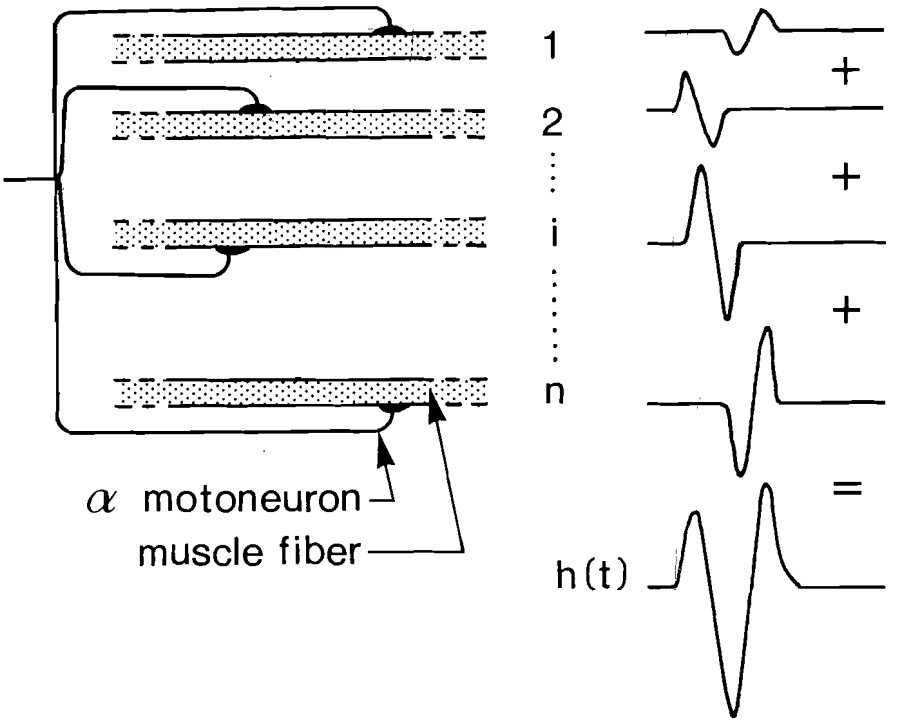
\includegraphics[width=0.75\linewidth]{./img/MUAP_oneMU.png}
	\end{center}
	\legend{Fonte: adaptado de \cite{Basmajian1985}.}
\end{figure}

Para os principais métodos utilizados em aquisição do sinal de EMG, é comum a captura da contribuição de mais de uma unidade motora no mesmo canal de aquisição. A influência de uma unidade motora na amplitude do sinal adquirido depende principalmente da distância das fibras musculares ao ponto de aquisição \cite{Gerdle1999}. Sinais de EMG de longa duração são constituídos por sequências temporais de MUAPs, também conhecidas como MUAPTs (\emph{MUAP Trains}). A Figura \ref{fig_MUAP_trains} exemplifica MUAPTs de diferentes MUs que somam-se para formar um sinal de EMG de longa duração.

\begin{figure}[htb]
	\caption{\label{fig_MUAP_trains}MUAPTs de diferentes MUs somam-se para compor o sinal adquirido por um canal de EMG.}
	\begin{center}
	    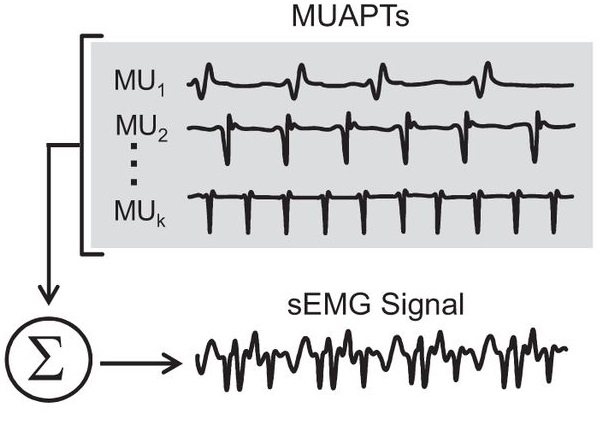
\includegraphics[width=0.75\linewidth]{./img/MUAP_trains.jpg}
	\end{center}
	\legend{Fonte: adaptado de \cite{Kline2014}}
\end{figure}

Para maiores detalhes sobre sinais de eletromiografia de superfície, conceitos sobre anatomia e fisiologia sugere-se a consulta de referências clássicas na área e adicionalmente as seguintes referências \cite{Favieiro2009}, \cite{Lopes2014} e \cite{Schons2014}.

%-------------------------------------------------------------------------
		\section{Métodos de Segmentação}
%-------------------------------------------------------------------------
\label{sec:MTDs}
Esta seção descreve os métodos de segmentação desenvolvidos, citando os trabalhos da área que foram utilizados como base teórica para os métodos.

Nota-se que nomes utilizados para variáveis e constantes (por exemplo, sinal a ser segmentado `$x$', \emph{threshold} `$T$', etc.) foram determinados pelo autor deste trabalho, não necessariamente sendo os mesmos utilizados nos trabalhos citados.

Para as definições dos Métodos 3 e 4 (MTD3 e MTD4) são utilizados os termos BEP (\emph{Beginning Extraction Point}, ponto inicial de um segmento) e EEP (\emph{Ending Extraction Point}, ponto final de um segmento), também utilizados em \cite{Pattichis1995}.
	
%-------------------------------------------------------------------------
				\subsection{Método 1 - método iterativo utilizando \emph{thresholding} para detecção de centros de segmentos de comprimento constante (MTD1)}
%-------------------------------------------------------------------------
Este método iterativo é adaptado do método de segmentação utilizado em \cite{Chauvet2001}. As definições da Tabela \ref{tab:mtd1params} serão utilizados para descrever este método.

\begin{table}[htb]
\IBGEtab{%
	\caption{Parâmetros utilizados para definir o MTD1.}%
	\label{tab_mtd1params}
}{%
	\begin{tabular}{ccc}
	\toprule
	Nome & Descrição \\
	\midrule \midrule
	$x$ & Sinal a ser segmentado \\
	\midrule
	$L$ & Comprimento total do sinal a ser segmentado \\
	\midrule
	$l$ & Comprimento desejado para os segmentos \\
	\midrule
	$T_k$ & Valor de \emph{threshold} para a iteração $k$ \\
	\midrule
	$T_{lim}$ & Valor de limite inferior para o \emph{threshold} \\
	\midrule 
	$q$ & Fração de $T_{k-1}$ para determinação de $T_k$ \\
	\midrule 
	$N_{k}$ & Número total de candidatos para centros de segmentos identificados na iteração $k$ \\
	\midrule 
	$r_k$ & Razão entre número de candidatos identificados na iteração $k$ e o comprimento total do sinal \\
	\midrule 
	$r_{target}$ & Razão mínima esperada para $r_k$, utilizada para determinar o final do método \\
	\bottomrule
\end{tabular}%
}{%
}
\end{table}


Inicialmente, determina-se o valor de \emph{threshold} $T_0$ equivalente ao máximo absoluto do sinal a ser segmentado $x$ (Equação (\ref{eq:mtd1t0})). O valor $T_k$ é atualizado em cada iteração $k$ como sendo uma fração $q$ de $T_{k-1}$ (Equação (\ref{eq:mtd1tk})). No trabalho de \cite{Chauvet2001}, este valor $q$ foi empiricamente determinado em 90\%.

\begin{equation}
\label{eq:mtd1t0}
  T_0 = max(x)
\end{equation}

\begin{equation}
\label{eq:mtd1tk}
  T_k = q \times T_{k-1}
\end{equation}

Pontos do sinal acima do valor de $T_k$ são possíveis candidatos para centros de segmentos. Caso exista mais de um possível candidato em uma vizinhança bilateral de $l$ amostras do sinal, apenas o ponto de maior amplitude nesta vizinhança é considerado. Para determinar o processo de finalização do método, avalia-se a razão $r_k$ entre a quantidade identificada de candidatos $N_{k}$ e o comprimento total do sinal $L$ (Equação (\ref{eq:mtd1rk})). Caso $r_k$ seja menor que um valor predeterminado $r_{target}$, calcula-se $T_{k+1}$ para realização da próxima iteração (Equação (\ref{eq:mtd1tk})). Caso $r_k$ seja maior ou igual ao valor predeterminado $r_{target}$, encerra-se o método e os segmentos são tomados como janelas de sinal de comprimento $l$, centradas nos candidatos identificados na última iteração.

\begin{equation}
\label{eq:mtd1rk}
  r_k = \frac{N_{k}}{L} 
\end{equation}

Adicionalmente, o estabelecimento de um valor limite mínimo para \emph{threshold} $T_{lim}$ garante que o método não entre em laço infinito e evita detecção de segmentos em trechos de baixa atividade muscular. Caso o valor de \emph{threshold} $T_k$ para a iteração atual seja inferior a $T_{lim}$, encerra-se o processo iterativo. O método de segmentação MTD1 é representado pelo fluxograma da Figura \ref{fig_mtd1flux}.

% Set up a few colours
\colorlet{lcfree}{green}
\colorlet{lcnorm}{blue}
\colorlet{lccong}{red}
% -------------------------------------------------
% Set up a new layer for the debugging marks, and make sure it is on
% top
\pgfdeclarelayer{marx}
\pgfsetlayers{main,marx}
% A macro for marking coordinates (specific to the coordinate naming
% scheme used here). Swap the following 2 definitions to deactivate
% marks.
\providecommand{\cmark}[2][]{%
  \begin{pgfonlayer}{marx}
    \node [nmark] at (c#2#1) {#2};
  \end{pgfonlayer}{marx}
  } 
\providecommand{\cmark}[2][]{\relax} 
% -------------------------------------------------
% Start the picture
\begin{figure}[htb]
	\caption{\label{fig_mtd1flux}Fluxograma representativo do MTD1.}
	\begin{center}
		\begin{tikzpicture}[%
			>=triangle 60,              % Nice arrows; your taste may be different
			start chain=going below,    % General flow is top-to-bottom
			node distance=6mm and 60mm, % Global setup of box spacing
			every join/.style={norm},   % Default linetype for connecting boxes
			]
		% ------------------------------------------------- 
		% A few box styles 
		% <on chain> *and* <on grid> reduce the need for manual relative
		% positioning of nodes
		\tikzset{
		  base/.style={draw, on chain, on grid, align=center, minimum height=4ex},
		  proc/.style={base, rectangle, text width=8em},
		  test/.style={base, diamond, aspect=2, text width=8em},
		  term/.style={proc, rounded corners},
		  % coord node style is used for placing corners of connecting lines
		  coord/.style={coordinate, on chain, on grid, node distance=6mm and 25mm},
		  % nmark node style is used for coordinate debugging marks
		  nmark/.style={draw, cyan, circle, font={\sffamily\bfseries}},
		  % -------------------------------------------------
		  % Connector line styles for different parts of the diagram
		  norm/.style={->, draw, lcnorm},
		  free/.style={->, draw, lcfree},
		  cong/.style={->, draw, lccong},
		  it/.style={font={\small\itshape}}
		}
		% -------------------------------------------------
		% Node placement: column 1
		\node [term, densely dotted, it, fill=lccong!25] (init) {INÍCIO};
		\node [proc, fill=lcnorm!25, join] {$k = 0$};
		\node [proc, fill=lcnorm!25, join] {$T_k = max(x)$};
		\node [proc, fill=lcnorm!25, join] (in) {$k \gets k + 1$};
		\node [proc, fill=lcnorm!25, join] {$T_k = q \times T_{k-1}$};
		\node [test, join] (t1) {$T_k < T_{min}$};
		\node [proc, fill=lcfree!25] (fin) {Segmentos de comprimento $l$ centrados nos candidatos identificados};
		\node [term, densely dotted, it, fill=lccong!25, join] {FIM};
		% -------------------------------------------------
		% Node placement: column 2
		\node [proc, fill=lcfree!25, right=of t1] (id) {Identificação de candidatos a centros de segmentos};
		\node [test, yshift=-0.2em, join] (t2) {$\frac{N_k}{L} \geq r_{target}$};
		% -------------------------------------------------
		% Test connections
		\path (t1.south) to node [near start, xshift=2em] {$sim$} (fin);
			\draw [*->,lcnorm] (t1.south) -- (fin);
			
		\path (t1.east) to node [near start, yshift=1em] {$não$} (id);
			\draw [o->,lcnorm] (t1.east) -- (id);
			
		\path (t2.west) to node [near start, yshift=1em] {$sim$} (fin);
			\draw [*->,lcnorm] (t2.west) -- (fin);
		
		\path (t2.east) to node [near start, xshift=6em, yshift=-3em] {$não$} (in);
			\draw [o->,lcnorm] (t2.east) |- (in);
		% -------------------------------------------------
		\end{tikzpicture}
	\end{center}
\end{figure}


%-------------------------------------------------------------------------
			\subsection{Método 2 - método não iterativo utilizando \emph{thresholding} para detecção de centros de segmentos de comprimento constante (MTD2)}
%-------------------------------------------------------------------------
Este é o método de segmentação utilizado por \cite{Katsis2006}, que será descrito pelas definições da Tabela \ref{tab:mtd2params}. Primeiramente, seleciona-se entre dois métodos de cálculo de \emph{threshold} $T$: ou utiliza-se $T$ como múltiplo da média aritmética do sinal $x$; ou $T$ é uma fração do valor máximo do sinal $x$. \cite{Katsis2006} utilizaram a relação do fluxograma da Figura \ref{fig_mtd2flux} para o cálculo de \emph{threshold} $T$.

\begin{table}[htb]
\IBGEtab{%
	\caption{Parâmetros utilizados para definir o MTD2.}%
	\label{tab:mtd2params}
}{%
	\begin{tabular}{ccc}
	\toprule
	Nome & Descrição \\
	\midrule \midrule
	$x$ & Sinal a ser segmentado \\
	\midrule
	$L$ & Comprimento total do sinal a ser segmentado \\
	\midrule
	$l$ & Comprimento desejado para os segmentos \\
	\midrule
	$T$ & Valor de \emph{threshold} \\
	\midrule
	$A$ & Coeficiente utilizado para decisão de método de cálculo de $T$ \\
	\midrule
	$B$ & Múltiplo da média aritmética do sinal $x$ para obtenção de $T$ \\
	\midrule
	$C$ & Fração do valor máximo do sinal $x$ para cálculo de $T$ \\
	\bottomrule
\end{tabular}%
}{%
}
\end{table}

\begin{figure}[!htb]
	\caption{\label{fig_mtd2flux} Fluxograma representativo do MTD2.}
	\begin{center}
		\begin{tikzpicture}[node distance = 2cm, auto]
			% Place nodes
			\node [block] (init) {INÍCIO};
			\node [decision, below = 1cm of init,text width=10em] (decide) {$max(x) > \frac{A}{L}\sum_{i=1}^{L}|x_i|$?};
			\node [block, below left = 1cm and 1cm of decide] (case 1) {$T = \frac{B}{L}\sum_{i=1}^{L}|x_i|$};
			\node [block, below right = 1cm and 1cm of decide] (case 2) {$T = \frac{max(x)}{C}$};
			\node [block, below = 3cm of decide] (identify) {Identificar centros de segmentos};
			\node [block, below = 1cm of identify] (stop) {Segmentos de comprimento $l$ nos centros identificados\\ \vspace{\onelineskip} FIM};
			
			% Draw edges
			\path [line] (init) -- (decide);
			\path [line] (decide) -| node [near start] {SIM} (case 1);
			\path [line] (decide) -| node [near start] {NÃO} (case 2);
			\path [line] (case 1) -| (identify);
			\path [line] (case 2) -| (identify);
			\path [line] (identify) -- (stop);
		\end{tikzpicture}
	\end{center}
\end{figure}


De forma similar ao MTD1, os pontos do sinal que tiverem valor acima de $T$ são considerados possíveis candidatos para centros de segmentos. Para os possíveis candidatos que estiverem afastados de uma distância inferior a $l$, apenas o candidato de maior amplitude é considerado. Em \cite{Katsis2006} foram utilizados coeficientes $A$, $B$ e $C$ respectivamente de 30, 5 e 5, com comprimento $l$ de 121 amostras.

%-------------------------------------------------------------------------
			\subsection{Método 3 - método com janela deslizante para detecção de BEP e EEP de segmentos utilizando variação total (MTD3)}
%-------------------------------------------------------------------------
Este é o método de segmentação utilizado em \cite{Gut2000}. As definições da Tabela \ref{tab:mtd3params} serão utilizados para descrever este método. Uma janela deslizante de comprimento $W$ percorre o sinal da esquerda para a direita. A cada incremento de $step$ amostras, caso a variação total $V$ (Equação (\ref{eq:varTotal})) do trecho de sinal contido pela janela exceda um limite $B$ (sendo $B > 0$), o ponto mais à esquerda da janela $w_0$ determina a BEP de um segmento. O EEP do correspondente segmento é então obtido como o ponto mais à direita ($w_0 + W$) da próxima janela na qual a variação total for menor que um limite $C$ (sendo $C < 0$). O MTD3 pode ser representado pelo fluxograma da Figura \ref{fig_mtd3flux}.

\begin{table}[htb]
\IBGEtab{%
	\caption{Parâmetros utilizados para definir o MTD3.}%
	\label{tab:mtd3params}
}{%
	\begin{tabular}{ccc}
	\toprule
	Nome & Descrição \\
	\midrule \midrule
	$x$ & Sinal a ser segmentado \\
	\midrule
	$W$ & Comprimento da janela deslizante utilizada pelo método \\
	\midrule
	$w_0$ & Número da amostra mais a esquerda da janela. Determina a posição instantânea da janela \\
	\midrule
	$\beta$ & Declividade média do sinal $x$ contido na janela deslizante \\
	\midrule
	$B$ & Valor limite para declividade média que determina um BEP\\
	\midrule
	$\gamma$ & Variação total do sinal $x$ contido na janela deslizante \\
	\midrule
	$C$ & Valor limite para variação total que determina um EEP\\
	\bottomrule
\end{tabular}%
}{%
}
\end{table}

\begin{equation}
\label{eq:varTotal}
	V = \sum\limits_{i=w_0+1}^{w_0+W} (x_i - x_{i-1})
\end{equation}

% Set up a few colours
\colorlet{lcfree}{green}
\colorlet{lcnorm}{blue}
\colorlet{lccong}{red}
% -------------------------------------------------
% Set up a new layer for the debugging marks, and make sure it is on
% top
\pgfdeclarelayer{marx}
\pgfsetlayers{main,marx}
% A macro for marking coordinates (specific to the coordinate naming
% scheme used here). Swap the following 2 definitions to deactivate
% marks.
\providecommand{\cmark}[2][]{%
  \begin{pgfonlayer}{marx}
    \node [nmark] at (c#2#1) {#2};
  \end{pgfonlayer}{marx}
  } 
\providecommand{\cmark}[2][]{\relax} 
% -------------------------------------------------
% Start the picture
\begin{figure}[!htb]
	\caption{\label{fig_mtd3flux}Fluxograma representativo do MTD3.}
	\begin{center}
		\begin{tikzpicture}[%
			>=triangle 60,              % Nice arrows; your taste may be different
			start chain=going below,    % General flow is top-to-bottom
			node distance=6mm and 60mm, % Global setup of box spacing
			every join/.style={norm},   % Default linetype for connecting boxes
			]
		% ------------------------------------------------- 
		% A few box styles 
		% <on chain> *and* <on grid> reduce the need for manual relative
		% positioning of nodes
		\tikzset{
		  base/.style={draw, on chain, on grid, align=center, minimum height=4ex},
		  proc/.style={base, rectangle, text width=10em},
		  test/.style={base, diamond, aspect=2, text width=6em},
		  term/.style={proc, rounded corners},
		  % coord node style is used for placing corners of connecting lines
		  coord/.style={coordinate, on chain, on grid, node distance=6mm and 25mm},
		  % nmark node style is used for coordinate debugging marks
		  nmark/.style={draw, cyan, circle, font={\sffamily\bfseries}},
		  % -------------------------------------------------
		  % Connector line styles for different parts of the diagram
		  norm/.style={->, draw, lcnorm},
		  free/.style={->, draw, lcfree},
		  cong/.style={->, draw, lccong},
		  it/.style={font={\small\itshape}}
		}
		% -------------------------------------------------
		% Node placement: column 1
		\node [term, densely dotted, it, fill=lccong!25] (init) {INÍCIO};
		\node [proc, fill=lcnorm!25, join] {$w_0 = 0$};
		\node [proc, fill=lcfree!25, join] (W) {Janela de comprimento $W$, iniciando em $w_0$};
		\node [proc, fill=lcnorm!25, join] (w0) {$w_0 \gets w_0 + 1$};
		\node [test, join] (t1) {$w_0 + W > L$};
		% -------------------------------------------------
		% Node placement: column 2
		\node [proc, fill=lcnorm!25, right=of t1] (beta) {$\beta = \frac{1}{W}\sum\limits_{i=w_0+1}^{w_0+W} (x_i - x_{i-1}) $};
		\node [test, join] (B) {$\beta > B$};
		\node [proc, fill=lcfree!25] (BEP) {$w_0$ é BEP};
		\node [proc, fill=lcnorm!25, join] (w01) {$w_0 \gets w_0 + 1$};
		\node [test, join] (t2) {$w_0 + W > L$};
		\node [proc, fill=lcnorm!25] (gamma) {$\gamma = \sum\limits_{i=w_0+1}^{w_0+W} (x_i - x_{i-1}) $};
		\node [test, join] (C) {$\gamma < C$};
		\node [proc, fill=lcfree!25] (EEP) {$w_0+W$ é EEP};
		% -------------------------------------------------
		% Node placement: column 1
		\node [proc, fill=lcfree!25, left=of gamma] (fin) {Segmentos limitados pelos BEPs e EEPs identificados};
		\node [term, densely dotted, it, fill=lccong!25, join] (fim) {FIM};
		% -------------------------------------------------
		% Coordinates
		\node [coord, right=of B, xshift = 4em] (c1) {};
		\node [coord, below=of t1, yshift = -17em] (c2) {};
		\node [coord, right=of C, xshift = 2em] (c3) {};
		% -------------------------------------------------
		% Test connections
		\path (t1.south) to node [near start, xshift=1em, yshift = 6em] {$sim$} (fin);
			\draw [*->,lcnorm] (t1.south) -- (c2) -- (fin);
		\path (t1.east) to node [near start, yshift=1em] {$não$} (beta);
			\draw [o->,lcnorm] (t1.east) -- (beta);
		\path (B.south) to node [near start, xshift=2em] {$sim$} (BEP);
			\draw [*->,lcnorm] (B.south) -- (BEP);
		\path (B.east) to node [near start, yshift=1em] {$não$} (c1);
			\draw [o->,lcnorm] (B.east) -- (c1);
		\path (t2.south) to node [near start, xshift=2em] {$não$} (gamma);
			\draw [o->,lcnorm] (t2.south) -- (gamma);
		\path (t2.west) to node [near start, yshift=1em] {$sim$} (c2);
			\draw [*->,lcnorm] (t2.west) -- (c2);
			\draw [->,lcnorm] (EEP) -| (c1) |- (w0);
		\path (C.south) to node [near start, xshift=2em] {$sim$} (EEP);
			\draw [*->,lcnorm] (C.south) -- (EEP);
		\path (C.east) to node [near start, yshift=1em] {$não$} (c3);
			\draw [o->,lcnorm] (C.east) -- (c3) |- (w01);
		% -------------------------------------------------
		\end{tikzpicture}
	\end{center}
\end{figure}


No método original de \cite{Gut2000}, BEPs foram detectadas pelo cálculo da declividade média $\beta$ no interior da janela (Equação (\ref{eq:decMedia})) nos pontos que excediam um limite $B$ (sendo $B > 0$), e EEPs pelo cálculo do módulo da variação total (Equação (\ref{eq:absVarTotal})) quando esta era menor que um limite $C$ (sendo $C > 0$).

\begin{equation}
\label{eq:decMedia}
	\beta = \frac{1}{W}\sum\limits_{i=w_0+1}^{w_0+W} (x_i - x_{i-1})
\end{equation}

\begin{equation}
\label{eq:absVarTotal}
	\gamma = \left|\sum\limits_{i=w_0+1}^{w_0+W} (x_i - x_{i-1})\right|
\end{equation}

Nota-se que $\gamma = |W\beta| = |V|$. O MTD3 proposto, ao utilizar apenas a Equação (\ref{eq:varTotal}) para detecção de BEPs e EEPs, explora tal relação para simplificar o método original, com a vantagem adicional de que os limites $B$ e $C$ passam a ser da mesma ordem de grandeza (com o método de \cite{Gut2000}, $B$ seria aproximadamente $W$ vezes menor que $C$).

O incremento de $step$ amostras (ao invés do avanço de $w_0$ de uma em uma amostra) serve para reduzir o número de vezes em que é necessário cálculo de variação total $V$, simplificando o processamento. Os limites de $l_{mín}$ e $l_{máx}$ são necessários para evitar identificação incorreta da EEP relacionada a uma BEP (i.e. $l_{máx}$ evita que o segmento BEP-EEP contenha sinal respectivo a mais de um movimento e $l_{mín}$ que o sinal seja segmentado em meio a um movimento).

%-------------------------------------------------------------------------
			\subsection{Método 4 - método com janela deslizante para detecção de BEP e EEP de segmentos utilizando \emph{thresholding} (MTD4)}
%-------------------------------------------------------------------------
Este método de segmentação é adaptado de \cite{Pattichis1995}. As definições da Tabela \ref{tab:mtd4params} serão utilizados para descrever este método.

\begin{table}[htb]
\IBGEtab{%
	\caption{Parâmetros utilizados para definir o MTD4.}%
	\label{tab:mtd4params}
}{%
	\begin{tabular}{ccc}
	\toprule
	Nome & Descrição \\
	\midrule \midrule
	$x$ & Sinal a ser segmentado \\
	\midrule
	$L$ & Comprimento total do sinal $x$ \\
	\midrule
	$W$ & Comprimento da janela deslizante utilizada pelo método \\
	\midrule
	$T$ & Valor de \emph{threshold} \\
	\bottomrule
\end{tabular}%
}{%
}
\end{table}

Uma janela deslizante de comprimento $W$, com início em $w_0$, percorre o sinal da esquerda para a direita. As BEPs de segmentos são os primeiros pontos $w_0$ em que o máximo valor de sinal $x$ contido na janela supera o valor de \emph{threshold} $T$. As EEPs associadas às BEPs são as posições $w_0 + W$ em que tal valor máximo volta a ser inferior a $T$. Assim como no MTD3, restrições para comprimento mínimo e máximo ($l_{mín}$ e $l_{máx}$) de segmentos são utilazadas. O fluxograma da Figura \ref{fig_mtd4flux} representa o MTD4.

% Set up a few colours
\colorlet{lcfree}{green}
\colorlet{lcnorm}{blue}
\colorlet{lccong}{red}
% -------------------------------------------------
% Set up a new layer for the debugging marks, and make sure it is on
% top
\pgfdeclarelayer{marx}
\pgfsetlayers{main,marx}
% A macro for marking coordinates (specific to the coordinate naming
% scheme used here). Swap the following 2 definitions to deactivate
% marks.
\providecommand{\cmark}[2][]{%
  \begin{pgfonlayer}{marx}
    \node [nmark] at (c#2#1) {#2};
  \end{pgfonlayer}{marx}
  } 
\providecommand{\cmark}[2][]{\relax} 
% -------------------------------------------------
% Start the picture
\begin{figure}[htb]
	\caption{\label{fig_mtd4flux}Fluxograma representativo do MTD4.}
	\begin{center}
		\begin{tikzpicture}[%
			>=triangle 60,              % Nice arrows; your taste may be different
			start chain=going below,    % General flow is top-to-bottom
			node distance=6mm and 60mm, % Global setup of box spacing
			every join/.style={norm},   % Default linetype for connecting boxes
			]
		% ------------------------------------------------- 
		% A few box styles 
		% <on chain> *and* <on grid> reduce the need for manual relative
		% positioning of nodes
		\tikzset{
		  base/.style={draw, on chain, on grid, align=center, minimum height=4ex},
		  proc/.style={base, rectangle, text width=10em},
		  test/.style={base, diamond, aspect=2, text width=7em},
		  term/.style={proc, rounded corners},
		  % coord node style is used for placing corners of connecting lines
		  coord/.style={coordinate, on chain, on grid, node distance=6mm and 25mm},
		  % nmark node style is used for coordinate debugging marks
		  nmark/.style={draw, cyan, circle, font={\sffamily\bfseries}},
		  % -------------------------------------------------
		  % Connector line styles for different parts of the diagram
		  norm/.style={->, draw, lcnorm},
		  free/.style={->, draw, lcfree},
		  cong/.style={->, draw, lccong},
		  it/.style={font={\small\itshape}}
		}
		% -------------------------------------------------
		% Node placement: column 1
		\node [term, densely dotted, it, fill=lccong!25] (init) {INÍCIO};
		\node [proc, fill=lcnorm!25, join] {$w_0 = 0$};
		\node [proc, fill=lcfree!25, join] (W) {Janela de comprimento $W$, iniciando em $w_0$};
		\node [proc, fill=lcnorm!25, join] (w0) {$w_0 \gets w_0 + step$};
		\node [test, join] (t1) {$w_0 + W > L$};
		% -------------------------------------------------
		% Node placement: column 2
		\node [test, fill=lcfree!25, right=of t1] (B) {Máximo do sinal contido na janela $> T$?};
		\node [proc, fill=lcfree!25] (BEP) {$w_0$ é BEP};
		\node [proc, fill=lcnorm!25, join] (w01) {$w_0 \gets w_0 + step$};
		\node [test, join] (t2) {$w_0+W > L$};
		\node [test] (lMax) {$w_0+W - BEP  > l_{máx}$};
		\node [test, fill=lcfree!25] (C) {Máximo do sinal contido na janela $< T$ e $w_0+W - BEP < l_{mín}$?};
		\node [proc, fill=lcfree!25] (EEP) {$w_0+W$ é EEP};
		% -------------------------------------------------
		% Node placement: column 3
		\node [proc, fill=lcfree!25, right=of lMax] (el) {Elimina último BEP identificado};
		% -------------------------------------------------
		% Node placement: column 1
		
		\node [proc, fill=lcfree!25, left=of gamma] (fin) {Pareamento de BEPs e EEPs identificados};
		\node [proc, fill=lcfree!25, join] {Segmentos limitados pelos BEPs e EEPs pareados};
		\node [term, densely dotted, it, fill=lccong!25, join] (fim) {FIM};
		% -------------------------------------------------
		% Coordinates
		\node [coord, right=of B, xshift = 15em] (c1) {};
		\node [coord, below=of c1, yshift = -20em] (c4) {};
		\node [coord, below=of t1, yshift = -13.1em] (c2) {};
		\node [coord, right=of C, xshift = 2em] (c3) {};
		% -------------------------------------------------
		% Test connections
		\path (t1.south) to node [near start, xshift=2em, yshift = 6em] {$sim$} (fin);
			\draw [*->,lcnorm] (t1.south) -- (c2) -- (fin);
		\path (t1.east) to node [near start, yshift=1em] {$não$} (B);
			\draw [o->,lcnorm] (t1.east) -- (B);
		\path (B.south) to node [near start, xshift=2em] {$sim$} (BEP);
			\draw [*->,lcnorm] (B.south) -- (BEP);
		\path (B.east) to node [near start, yshift=1em, xshift=-2em] {$não$} (c1);
			\draw [o->,lcnorm] (B.east) -- (c1);
		\path (t2.south) to node [near start, xshift=2em] {$não$} (lMax);
			\draw [o->,lcnorm] (t2.south) -- (lMax);
		\path (t2.west) to node [near start, yshift=1em] {$sim$} (c2);
			\draw [*->,lcnorm] (t2.west) -- (c2);
			\draw [->,lcnorm] (EEP) -| (c1) |- (w0);
		\path (C.south) to node [near start, xshift=2em] {$sim$} (EEP);
			\draw [*->,lcnorm] (C.south) -- (EEP);
		\path (C.east) to node [near start, xshift=2em] {$não$} (c3);
			\draw [o->,lcnorm] (C.east) -- (c3) |- (w01);
		\path (lMax.east) to node [near start, yshift=1em] {$sim$} (el);
			\draw [*->,lcnorm] (lMax.east) -- (el);
			\draw [->,lcnorm] (el) -- (c4);
		\path (lMax.south) to node [near start, xshift=2em] {$não$} (C);
			\draw [o->,lcnorm] (lMax.south) -- (C);
		% -------------------------------------------------
		\end{tikzpicture}
	\end{center}
\end{figure}


%-------------------------------------------------------------------------
		\section{Princípios Básicos sobre Redes Neurais Artificiais}
%-------------------------------------------------------------------------
Rede Neural Artificial (RNA) trata-se de um método computacional que, inspirado nos modelos de redes neurais biológicas, ``aprende'' a resolver determinados problemas \cite{YEGNANARAYANA2009}, apresentando aplicações em diversos tipos de sinais (e.g. sinais de áudio, imagem e, como é o caso deste trabalho, eletromiografia).

Propostas de utilização de RNA com sinais de EMG para classificação de movimentos datam antes de 1990, a exemplo do trabalho de \cite{Hiraiwa1989}, que menciona a vantagem de RNA sobre outros mecanismos de aprendizado computacional na classificação de padrões que não apresentam separabilidade linear. Desde então, múltiplos trabalhos na área já utilizaram RNA para classificação de movimentos utilizando EMG (e.g. \cite{Hudgins1993}, \cite{Subasi2006}, \cite{Bu2003}), apresentando resultados satisfatórios para taxa de acerto de classificação.

%-------------------------------------------------------------------------
			\subsection{Modelo Matemático de RNAs}
%-----------------------------------------------------------------------

Uma RNA é modelada pelas comunicações de um conjunto de ``neurônios'' artificiais. Cada neurônio artificial, como mostrado na Figura \ref{fig:neuron}, trata-se de uma função matemática que soma de forma ponderada $n$ entradas com pesos $w_n$ e um valor de \emph{bias} $B$ e utiliza o resultado desta soma em uma função dita ``função de ativação'' \cite{Tanikic2012}.

%------------------------------------------------------------------------------		
% Styles:
%------------------------------------------------------------------------------
\tikzstyle{io} = [circle, minimum width=0.1cm, draw=black, fill=black]
\tikzstyle{sum} = [circle, minimum width=1cm, draw=black]
\tikzstyle{func}= [rectangle, minimum width=1cm, minimum height=1cm, draw=black]

\begin{figure}[htb]
	\caption{\label{fig:neuron} Diagrama representativo do modelo de um neurônio artificial genérico.}
	\begin{center}
		\begin{tikzpicture}[>=triangle 60]
%------------------------------------------------------------------------------
% Node placement
%------------------------------------------------------------------------------
			\node[io](x1){}; \node[left=of x1, xshift=2em]{$in_1$};
			\node[io, below=of x1](x2){}; \node[left=of x2, xshift=2em]{$in_2$};
			\node[io, below=of x2](x3){}; \node[left=of x3, xshift=2em]{$in_3$};
			\node[below=of x3, yshift=2em]{...};			
			\node[io, below=of x3](xn){}; \node[left=of xn, xshift=2em]{$in_n$};
			
			\node[sum, right=of x2, xshift = 2em, yshift = -1.5em](sum){$\sum$};
			
			\node[io, below=of sum](B){}; \node[right=of B, xshift=-2em]{B};
			
			\node[func, right=of sum](f){$f$}; \node[above=of f, align=left, yshift=-2em]{Função de \\ Ativação};
			
			\node[right=of f](out){}; \node[right=of out, xshift=-3em]{$out$};
			
%------------------------------------------------------------------------------
% Connections
%------------------------------------------------------------------------------
			\draw [->,black] (x1) -- (sum);
			\path (x1) to node [near start, xshift=1em]{$w_1$}(sum);
			
			\draw [->,black] (x2) -- (sum);                                
			\path (x2) to node [near start, xshift=1em, yshift=0.3em]{$w_2$}(sum);
			
			\draw [->,black] (x3) -- (sum);                                
			\path (x3) to node [near start, xshift=1em, yshift=-0.1em]{$w_3$}(sum);
			
			\draw [->,black] (xn) -- (sum);                                
			\path (xn) to node [near start, xshift=1em]{$w_n$}(sum);
			
			\draw [->,black] (B) -- (sum);
			\draw [->,black] (sum) -- (f);
			\draw [->,black] (f) -- (out);

		\end{tikzpicture}
	\end{center}
	\legend{Fonte: adaptado de \citeonline{Tanikic2012}}
\end{figure}


As RNAs utilizadas neste trabalho apresentam arquitetura chamada \emph{feedforward}, onde neurônios são estruturados em camadas consecutivas, de forma que neurônios de uma mesma camada recebem as saídas de neurônios da camada anterior. A Figura \ref{fig:feedforward} exemplifica a estrutura de uma rede neural \emph{feedforward} que utiliza $m$ entradas para produzir $n$ saídas, utilizando duas camadas de neurônios chamadas de ``camadas ocultas'' (i.e. a saída da camada é utilizada como entrada da próxima camada) e uma camada de saída.

%------------------------------------------------------------------------------		
% Styles:
%------------------------------------------------------------------------------
\tikzstyle{io} = [circle, minimum width=0.1cm, draw=black, fill=black]
\tikzstyle{neuron} = [circle, minimum width=1cm, draw=black]
\tikzstyle{section} = [rectangle, minimum width=2cm, densely dotted, very thick]

\begin{figure}[htb]
	\caption{\label{fig:feedforward} Exemplo de uma RNA em arquitetura \emph{feedforward}.}
	\begin{center}
		\begin{tikzpicture}[>=triangle 60]
%------------------------------------------------------------------------------
% Node placement
%------------------------------------------------------------------------------
			\node[io](x1){}; \node[left=of x1](x1in){$in_1$};
			\node[io, below=of x1](x2){}; \node[left=of x2](x2in){$in_2$};
			\node[io, below=of x2](x3){}; \node[left=of x3](x3in){$in_3$};
			\node[below=of x3, yshift=2em]{...};
			\node[io, below=of x3](x4){}; \node[left=of x4](x4in){$in_m$};

			\node[neuron, right=of x1, xshift=2em, yshift=2em](n1){$N_1$};
			\node[neuron, below=of n1](n2){$N_2$};
			\node[neuron, below=of n2](n3){$N_3$};
			\node[below=of n3, yshift=2em]{...};
			\node[neuron, below=of n3](n4){$N_r$};
			
			\node[neuron, right=of n1, xshift=2em](ns1){$N_1$};
			\node[neuron, below=of ns1](ns2){$N_2$};
			\node[neuron, below=of ns2](ns3){$N_3$};
			\node[below=of ns3, yshift=2em]{...};
			\node[neuron, below=of ns3](ns4){$N_s$};
			
			\node[neuron, right=of ns1, xshift=2em, yshift=-2em](nt1){$N_1$};
			\node[neuron, below=of nt1](nt2){$N_2$};
			\node[below=of nt2, yshift=2em]{...};
			\node[neuron, below=of nt2](nt3){$N_n$};
			
			\node[right=of nt1](y1){$out_1$};
			\node[right=of nt2](y2){$out_2$};
			\node[right=of nt3](y3){$out_n$};
			
			\node[section, above=of n1,  minimum height=7.2cm, yshift=-8.1cm, draw=red](s1){};
			\node[below=of s1, align=left, yshift=2em]{Primeira \\ Camada \\ Oculta};
			\node[section, above=of ns1,  minimum height=7.2cm, yshift=-8.1cm, draw=green](s2){};
			\node[below=of s2, align=left, yshift=2em]{Segunda \\ Camada \\ Oculta};
			\node[section, above=of nt1,  minimum height=5.2cm, yshift=-6.1cm, draw=blue](s3){};
			\node[below=of s3, align=left, yshift=2em]{Camada \\ de Saída};

%------------------------------------------------------------------------------
% Connections
%------------------------------------------------------------------------------
			\draw [->,black] (x1in) -- (x1);
			\draw [->,black] (x2in) -- (x2);
			\draw [->,black] (x3in) -- (x3);
			\draw [->,black] (x4in) -- (x4);

			\draw [->,black] (x1) -- (n1);
			\draw [->,black] (x1) -- (n2);
			\draw [->,black] (x1) -- (n3);
			\draw [->,black] (x1) -- (n4);
			\draw [->,black] (x2) -- (n1);
			\draw [->,black] (x2) -- (n2);
			\draw [->,black] (x2) -- (n3);
			\draw [->,black] (x2) -- (n4);
			\draw [->,black] (x3) -- (n1);
			\draw [->,black] (x3) -- (n2);
			\draw [->,black] (x3) -- (n3);
			\draw [->,black] (x3) -- (n4);
			\draw [->,black] (x4) -- (n1);
			\draw [->,black] (x4) -- (n2);
			\draw [->,black] (x4) -- (n3);
			\draw [->,black] (x4) -- (n4);

			\draw [->,black] (n1) -- (ns1);
			\draw [->,black] (n1) -- (ns2);
			\draw [->,black] (n1) -- (ns3);
			\draw [->,black] (n1) -- (ns4);
			\draw [->,black] (n2) -- (ns1);
			\draw [->,black] (n2) -- (ns2);
			\draw [->,black] (n2) -- (ns3);
			\draw [->,black] (n2) -- (ns4);
			\draw [->,black] (n3) -- (ns1);
			\draw [->,black] (n3) -- (ns2);
			\draw [->,black] (n3) -- (ns3);
			\draw [->,black] (n3) -- (ns4);
			\draw [->,black] (n4) -- (ns1);
			\draw [->,black] (n4) -- (ns2);
			\draw [->,black] (n4) -- (ns3);
			\draw [->,black] (n4) -- (ns4);
			
			\draw [->,black] (ns1) -- (nt1);
			\draw [->,black] (ns1) -- (nt2);
			\draw [->,black] (ns1) -- (nt3);
			\draw [->,black] (ns2) -- (nt1);
			\draw [->,black] (ns2) -- (nt2);
			\draw [->,black] (ns2) -- (nt3);
			\draw [->,black] (ns3) -- (nt1);
			\draw [->,black] (ns3) -- (nt2);
			\draw [->,black] (ns3) -- (nt3);
			\draw [->,black] (ns4) -- (nt1);
			\draw [->,black] (ns4) -- (nt2);
			\draw [->,black] (ns4) -- (nt3);
		
			\draw [->,black] (nt1) -- (y1);
			\draw [->,black] (nt2) -- (y2);
			\draw [->,black] (nt3) -- (y3);
			
		\end{tikzpicture}
	\end{center}
%	\legend{Fonte: adaptado de \cite{BARBOSA2005}}
\end{figure}


\cite{Hornik1991} mostra que ao utilizar neurônios com função de ativação contínua, limitada e não constante, a taxa de acerto de classificação para uma RNA de arquitetura \emph{feedforward} depende somente do número de neurônios artificiais utilizados nas camadas ocultas. Em aplicações de reconhecimento de padrões, normalmente utiliza-se uma função de ativação do tipo sigmoide (i.e. função cuja curva lembra a forma de um ``S'').  A função de ativação utilizada para RNAs, neste trabalho, é a função sigmoide logística $logsig()$, dada pela Equação (\ref{eq:logsig}).

\begin{equation}
\label{eq:logsig}
	logsig(x) = \frac{1}{1+e^{-x}}
\end{equation}

%-------------------------------------------------------------------------
			\subsection{Treinamento de RNAs}
%-----------------------------------------------------------------------

Uma RNA pode ser utilizada para resolver determinado problema após um processo de treinamento supervisionado. Conjuntos de dados de treinamento (entradas e respostas esperadas) são apresentados à RNA. Um algoritmo iterativo modifica os pesos e \emph{bias} dos neurônios buscando combinação que otimize o desempenho da RNA para os dados de treinamento. Às iterações do algoritmo de treinamento, em que os dados de treinamento são reapresentados à RNA, dá-se o nome de \emph{epoch}. O algoritmo utilizado para treinamento de RNAs, neste trabalho, chama-se \emph{scaled conjugate gradient backpropagation} \cite{Moller1993} (identificado em MATLAB como \emph{trainscg}), que apresenta boa performance em problemas de reconhecimento de padrões.

Quando uma RNA é aplicada para classificação de séries temporais de sinais, as entradas (chamadas ``preditores'') utilizadas pela RNA são características extraídas de um trecho do sinal (e.g. número de cruzamentos por zero, valor médio, valor RMS). A extração de características tem o objetivo de reduzir a dimensionalidade do vetor de entradas da RNA (i.e. ao invés de um trecho de sinal com grande número de amostras, a entrada da RNA trata-se de um número arbitrariamente pequeno de preditores), o que apresenta vantagens em desempenho computacional e contorna problemas que surgem da classificação de sinais ruidosos \cite{Kim2000}.

Para maiores detalhes sobre RNAs e outros métodos de aprendizado computacional, sugere-se consulta das seguintes referências. \cite{YEGNANARAYANA2009}, \cite{Abraham2005} e \cite{Drew20003}.

%-------------------------------------------------------------------------
			\subsection{Valor $F$}
%-------------------------------------------------------------------------
Em análises de sistemas classificadores, costumeiramente utiliza-se uma tabela conhecida como ``matriz de confusão''. A Tabela \ref{tab:conf_example} exemplifica uma matriz de confusão de um classificador dito ``binário'' (i.e. resultados de classificação possíveis pertencem a duas classes - ``positiva'' ou ``negativa'').

\begin{table}[htb]
\IBGEtab{%
	\caption{Exemplo de matriz de confusão.}%
	\label{tab:conf_example}
}{%
	\begin{tabular}{cc|c|c}
	\toprule
	&&\multicolumn{2}{c}{Classificação obtida}\\
	\midrule
	&& Negativa & Positiva\\
	\midrule \midrule
	Classificação&Negativa&$a$&$b$\\
	\cline{2-4}
	esperada&Positiva&$c$&$d$\\
	\bottomrule
\end{tabular}%
}{%
	$a$: verdadeiros negativos\\
	$b$: falsos positivos     \\
	$c$: falsos negativos     \\
	$d$: verdadeiros positivos\\
	Fonte: adaptado de \cite{Kubat1998}.
}
\end{table}

Extrapolar a Tabela \ref{tab:conf_example} para o caso das RNAs deste trabalho, que realizam classificação entre 17 classes de movimentos, significa obter tabela equivalente (com respectivos valores $a$, $b$, $c$ e $d$) para cada uma das classes de movimento, interpretando caso ``Positiva'' como a ocorrência da classe de movimento e ``Negativa'' a não-ocorrência da mesma.

Em situações onde existe grande disparidade entre número de classes esperadas positivas e negativas, é comum o uso dos indicadores de precisão $p$ (Equação(\ref{eq:precisao})) e sensitividade $r$ (Equação(\ref{eq:sensitividade})) - que não utilizam em suas definições o número geralmente grande de verdadeiros negativos $a$ - e combinações destes indicadores \cite{Kubat1998}. O valor $F$, por exemplo, é definido como a média harmônica entre precisão e senstividade, conforme a Equação (\ref{eq:fscore}). Para avaliação de desempenho de classificação de RNAs, este trabalho utilizará o valor $F$.

\begin{equation}
\label{eq:precisao}
	p = \frac{d}{b+d}
\end{equation}

\begin{equation}
\label{eq:sensitividade}
	r = \frac{d}{c+d}
\end{equation}

\begin{equation}
\label{eq:fscore}
	F = 2 \times \frac{p \times r}{p+r}
\end{equation}

%=========================================================================
% METODOLOGIA EXPERIMENTAL
	\chapter{Metodologia Experimental}
%=========================================================================

%=========================================================================
		\section{Bases de Dados Utilizadas}
%=========================================================================
Este trabalho faz uso de aquisições para o exercício 1 da base de dados número 2 do projeto NinaPro \cite{Gijsberts2014} e a base de dados em construção realizada pelo Laboratório de Instrumentação Eletro-Eletrônica (IEE).

A base de dados do IEE busca replicar os métodos de aquisição utilizados pelo projeto NinaPro, contando com os mesmos movimentos realizados, mesmo posicionamento de eletrodos e mesmo período de amostragem (500 $\mu s$). A base de dados NinaPro número 2 é composta por sinais de aquisição com 40 voluntários, enquanto a base de dados do IEE, ainda em construção, contém atualmente sinais de 10 voluntários.

%-------------------------------------------------------------------------
			\subsection{Posicionamento de Eletrodos}
%-------------------------------------------------------------------------
Os sinais de EMG de superfície para ambas as bases utilizadas neste trabalho são compostos por canais de aquisição de 12 eletrodos posicionados no braço direito de voluntários saudáveis (i.e. não amputados e sem desordens neuromusculares). Os primeiros 8 canais correspondem a eletrodos posicionados de forma a circundar o antebraço e a junção úmero-radial. O eletrodo do canal número 9 é posicionado sobre o músculo flexor superfícial dos dedos e o eletrodo do canal 10, em oposição, é posicionado sobre o músculo extensor dos dedos. Os últimos dois eletrodos, 11 e 12, são posicionados sobre o bíceps e o tríceps, respectivamente. A Figura \ref{fig:eletrodos} apresenta o posionamento para os doze eletrodos de superfície e a numeração de seus respectivos canais que compõem os sinais para ambas as bases de dados.

\begin{figure}[htb]
	\caption{\label{fig:eletrodos}Posicionamento de eletrodos de superfície no braço de um voluntário.}
	\begin{center}
	    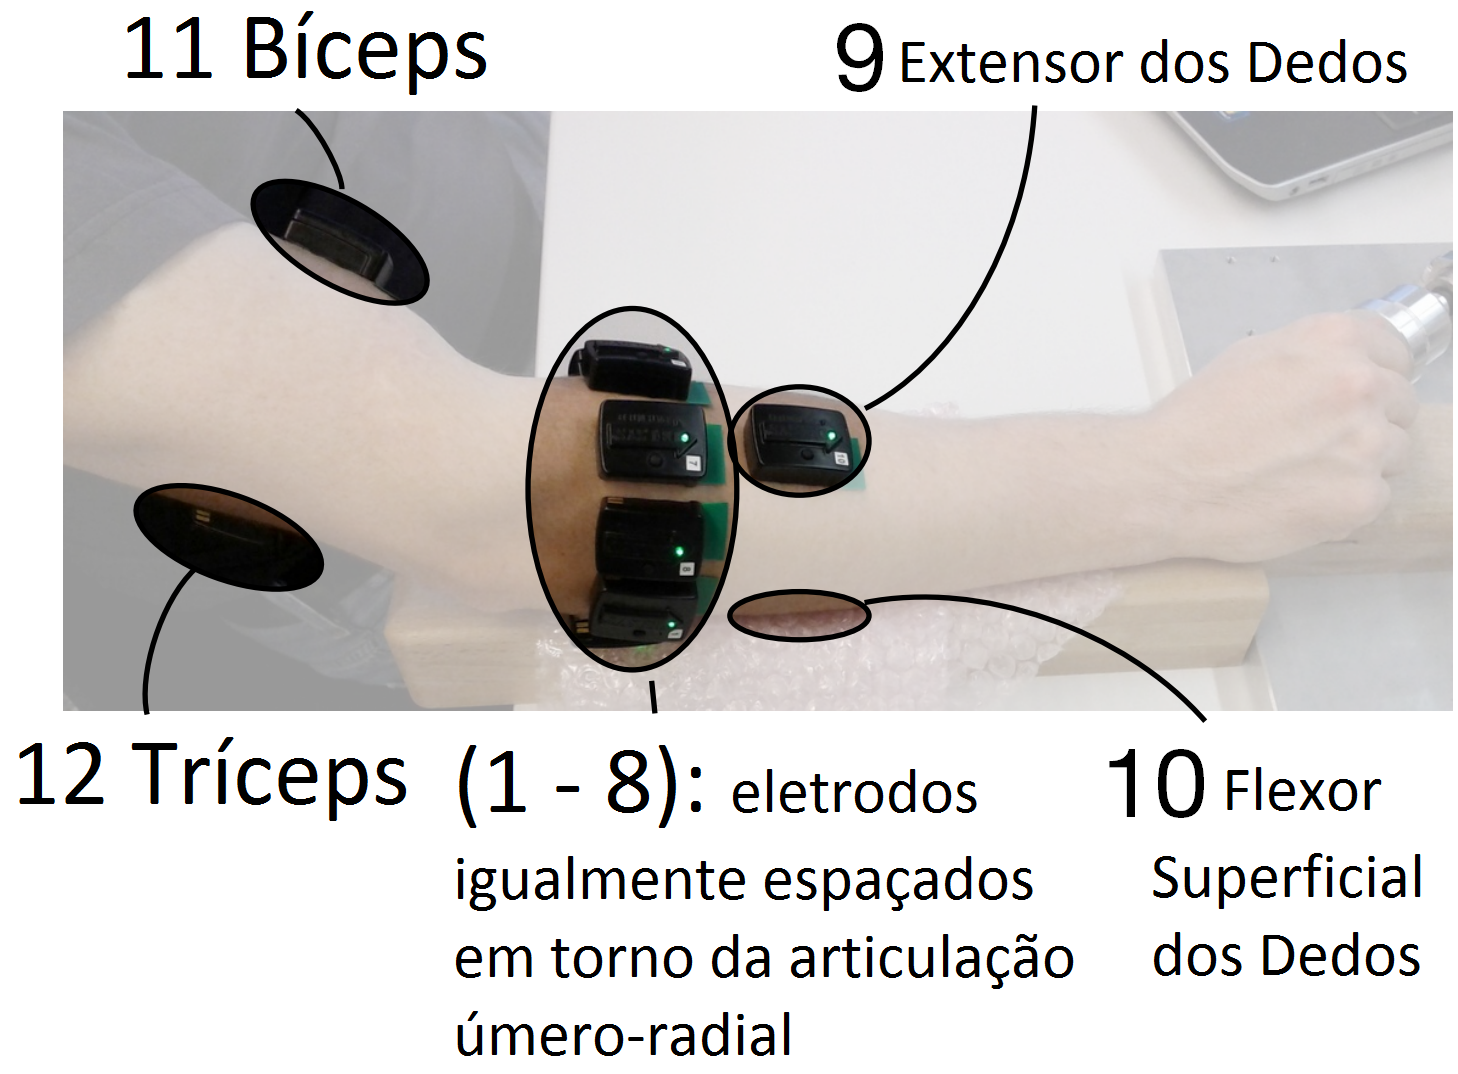
\includegraphics[width=0.75\linewidth]{./img/eletrodos.png}
	\end{center}
	\legend{Fonte: adaptado de \cite{Gijsberts2014}}
\end{figure}

%-------------------------------------------------------------------------
			\subsection{Sistema para Aquisição de EMGs no IEE}
%-------------------------------------------------------------------------
Para aquisições realizadas no IEE, os eletrodos são conectados a dois sistemas de aquisição EMG 830C, produzidos pela empresa ``EMG \emph{System} do Brasil'', de oito canais cada (os canais de número 1 a 8, que circundam a junção úmero-radial, são conectados ao primeiro sistema e os canais 9 a 12 ao segundo sistema). Os sinais de referência para os canais são tomados de eletrodos posicionados na testa do volutário.

Os sistemas EMG 830C são conectados a um computador pelo conjunto de \emph{Data Acquisition} (DAQ) NI SCB-68A e NI USB-6289. O computador executa uma rotina de aquisição de sinais implementada em NI LabView que é também responsável por exibir um vídeo com movimentos a serem replicados pelo voluntário. O diagrama da Figura \ref{fig:daq} resume o sistema de aquisição para a base de dados do IEE.

% Set up a few colours
\colorlet{lcfree}{green}
\colorlet{lcnorm}{blue}
\colorlet{lccong}{red}
% -------------------------------------------------
% Set up a new layer for the debugging marks, and make sure it is on
% top
\pgfdeclarelayer{marx}
\pgfsetlayers{main,marx}
% A macro for marking coordinates (specific to the coordinate naming
% scheme used here). Swap the following 2 definitions to deactivate
% marks.
\providecommand{\cmark}[2][]{%
  \begin{pgfonlayer}{marx}
    \node [nmark] at (c#2#1) {#2};
  \end{pgfonlayer}{marx}
  } 
\providecommand{\cmark}[2][]{\relax} 
% -------------------------------------------------
% Start the picture
\begin{figure}[htb]
	\caption{\label{fig:daq} Diagrama de blocos para o sistema de aquisição da base de dados do IEE.}
	\begin{center}
		\begin{tikzpicture}[%
			>=triangle 60,              % Nice arrows; your taste may be different
			start chain=going below,    % General flow is top-to-bottom
			node distance=6mm and 60mm, % Global setup of box spacing
			every join/.style={norm},   % Default linetype for connecting boxes
			]
		% ------------------------------------------------- 
		% A few box styles 
		% <on chain> *and* <on grid> reduce the need for manual relative
		% positioning of nodes
		\tikzset{
		  base/.style={draw, on chain, on grid, align=center, minimum height=4ex},
		  proc/.style={base, rectangle, text width=4cm},
		  test/.style={base, diamond, aspect=2, text width=8em},
		  term/.style={proc, rounded corners},
		  % coord node style is used for placing corners of connecting lines
		  coord/.style={coordinate, on chain, on grid, node distance=6mm and 25mm},
		  % nmark node style is used for coordinate debugging marks
		  nmark/.style={draw, cyan, circle, font={\sffamily\bfseries}},
		  % -------------------------------------------------
		  % Connector line styles for different parts of the diagram
		  norm/.style={->, draw, lcnorm},
		  free/.style={->, draw, lcfree},
		  cong/.style={->, draw, lccong},
		  it/.style={font={\small\itshape}}
		}
		% -------------------------------------------------
		% Node placement: column 1
		\node [proc, fill=lcfree!25] (eletrodos) {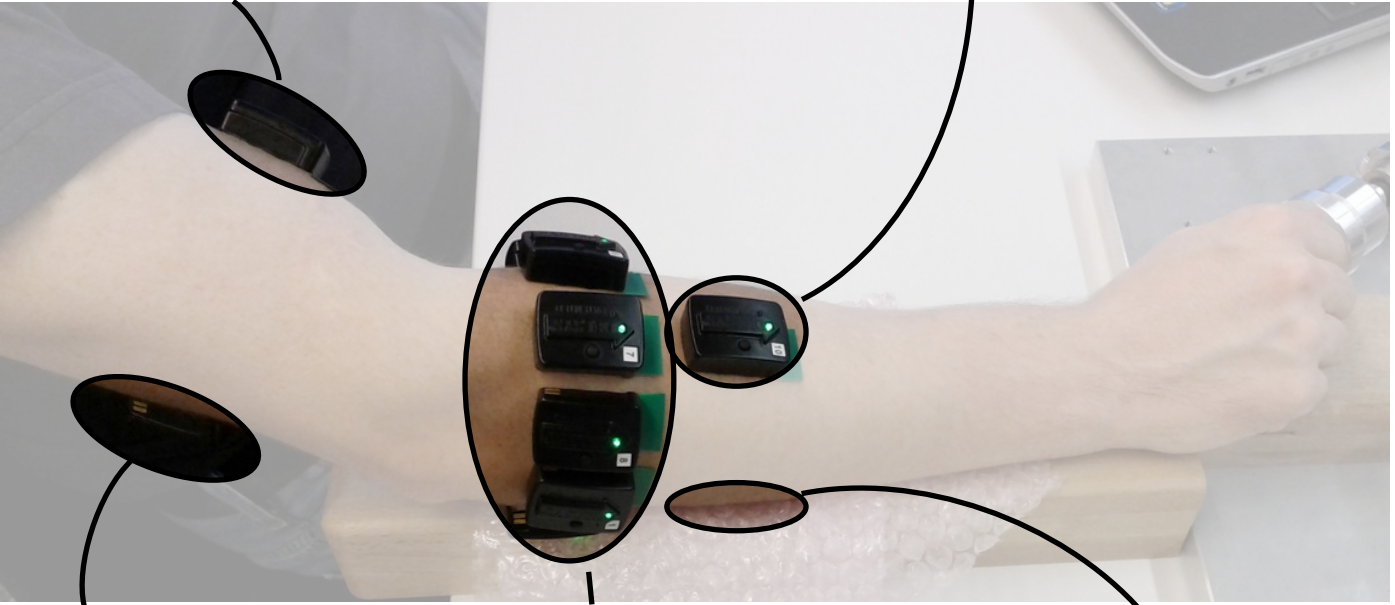
\includegraphics[width=4cm]{./img/eletrodos2.png}};
		\node [above=of eletrodos, yshift=-1.5em] {Eletrodos};
		\node [proc, fill=lcnorm!25, right=of eletrodos, yshift=4em] (EMG1) {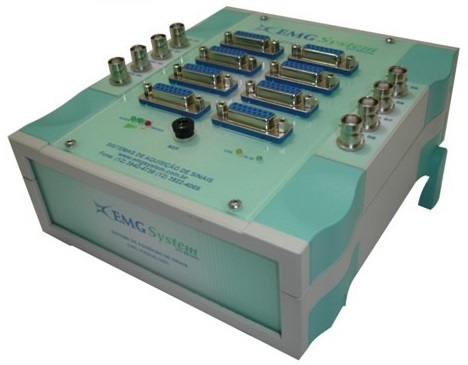
\includegraphics[width=3cm]{./flowcharts/EMG_830_C.jpg}};
		\node [proc, fill=lcnorm!25, right=of eletrodos, yshift=-4em] (EMG2) {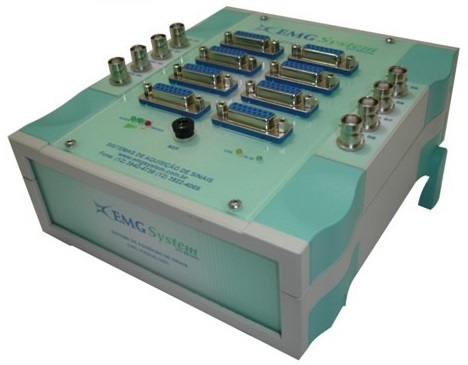
\includegraphics[width=3cm]{./flowcharts/EMG_830_C.jpg}};
		\node [above=of EMG2, yshift=-1.5em] {EMG 830C};
		\node [proc, fill=lccong!25, right=of EMG2, yshift=4em] (NI) {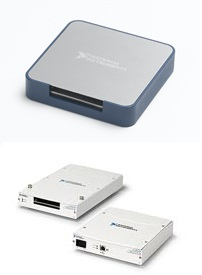
\includegraphics[width=3cm]{./flowcharts/ni_daq.jpg}};
		\node [above=of NI, yshift=-1.5em] {NI DAQ (SCB-68A e USB-6289)};
		\node [below=of NI] (labview) {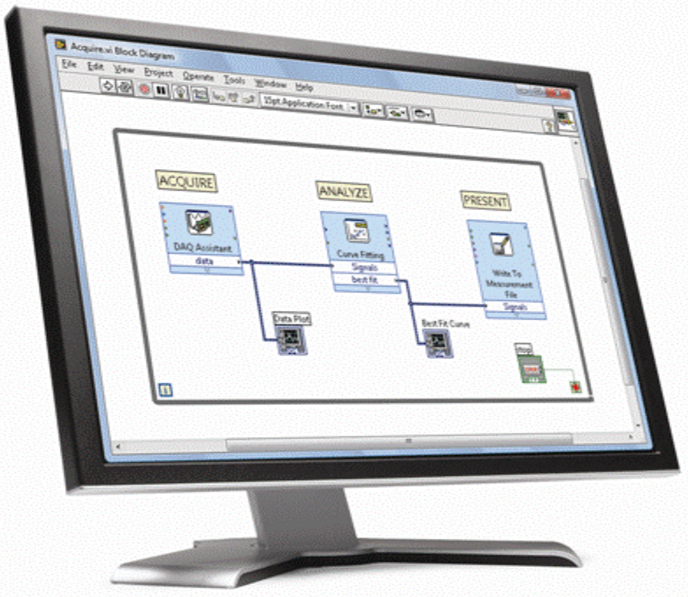
\includegraphics[width=3cm]{./img/labview.png}};
		\node [left=of labview, xshift=15em] {NI LabView};
		% -------------------------------------------------
%------------------------------------------------------------------------------
% Connections
%------------------------------------------------------------------------------
			\draw [->,black] (eletrodos) -- (EMG1);
			\path (eletrodos) to node [near start, yshift=2em, xshift=1em, align=center]{Canais \\ 1 a 8}(EMG1);
			\draw [->,black] (eletrodos) -- (EMG2);
			\path (eletrodos) to node [near start, yshift=-2em, xshift=1em, align=center]{Canais \\ 9 a 12}(EMG2);
			\draw [->,black] (EMG1) -- (NI);
			\draw [->,black] (EMG2) -- (NI);
			\draw [->,black] (NI) -- (labview);
		\end{tikzpicture}
	\end{center}
	\legend{Fonte: montagem com imagens de \cite{Gijsberts2014} e dos \emph{websites} das empresas EMG \emph{Systems} do Brasil e \emph{National Instruments}}.
\end{figure}


%-------------------------------------------------------------------------
			\subsection{Movimentos de Interesse}
%-------------------------------------------------------------------------
Após o posicionamento de eletrodos, os voluntários sentam-se em frente a um monitor e apoiam o braço direito de forma relaxada sobre uma superfície horizontal próxima à altura do cotovelo. O monitor exibe um vídeo com uma mão direita, digitalmente animada, realizando movimentos de interesse que devem ser replicados pelos voluntários. A Figura \ref{fig:video} apresenta a mão digitalmente animada realizando alguns dos movimentos de interesse deste trabalho.

\begin{figure}[htb]
	\caption{\label{fig:video}Cenas do vídeo apresentado aos voluntários na aquisição do Laboratório IEE.}
	\begin{center}
	    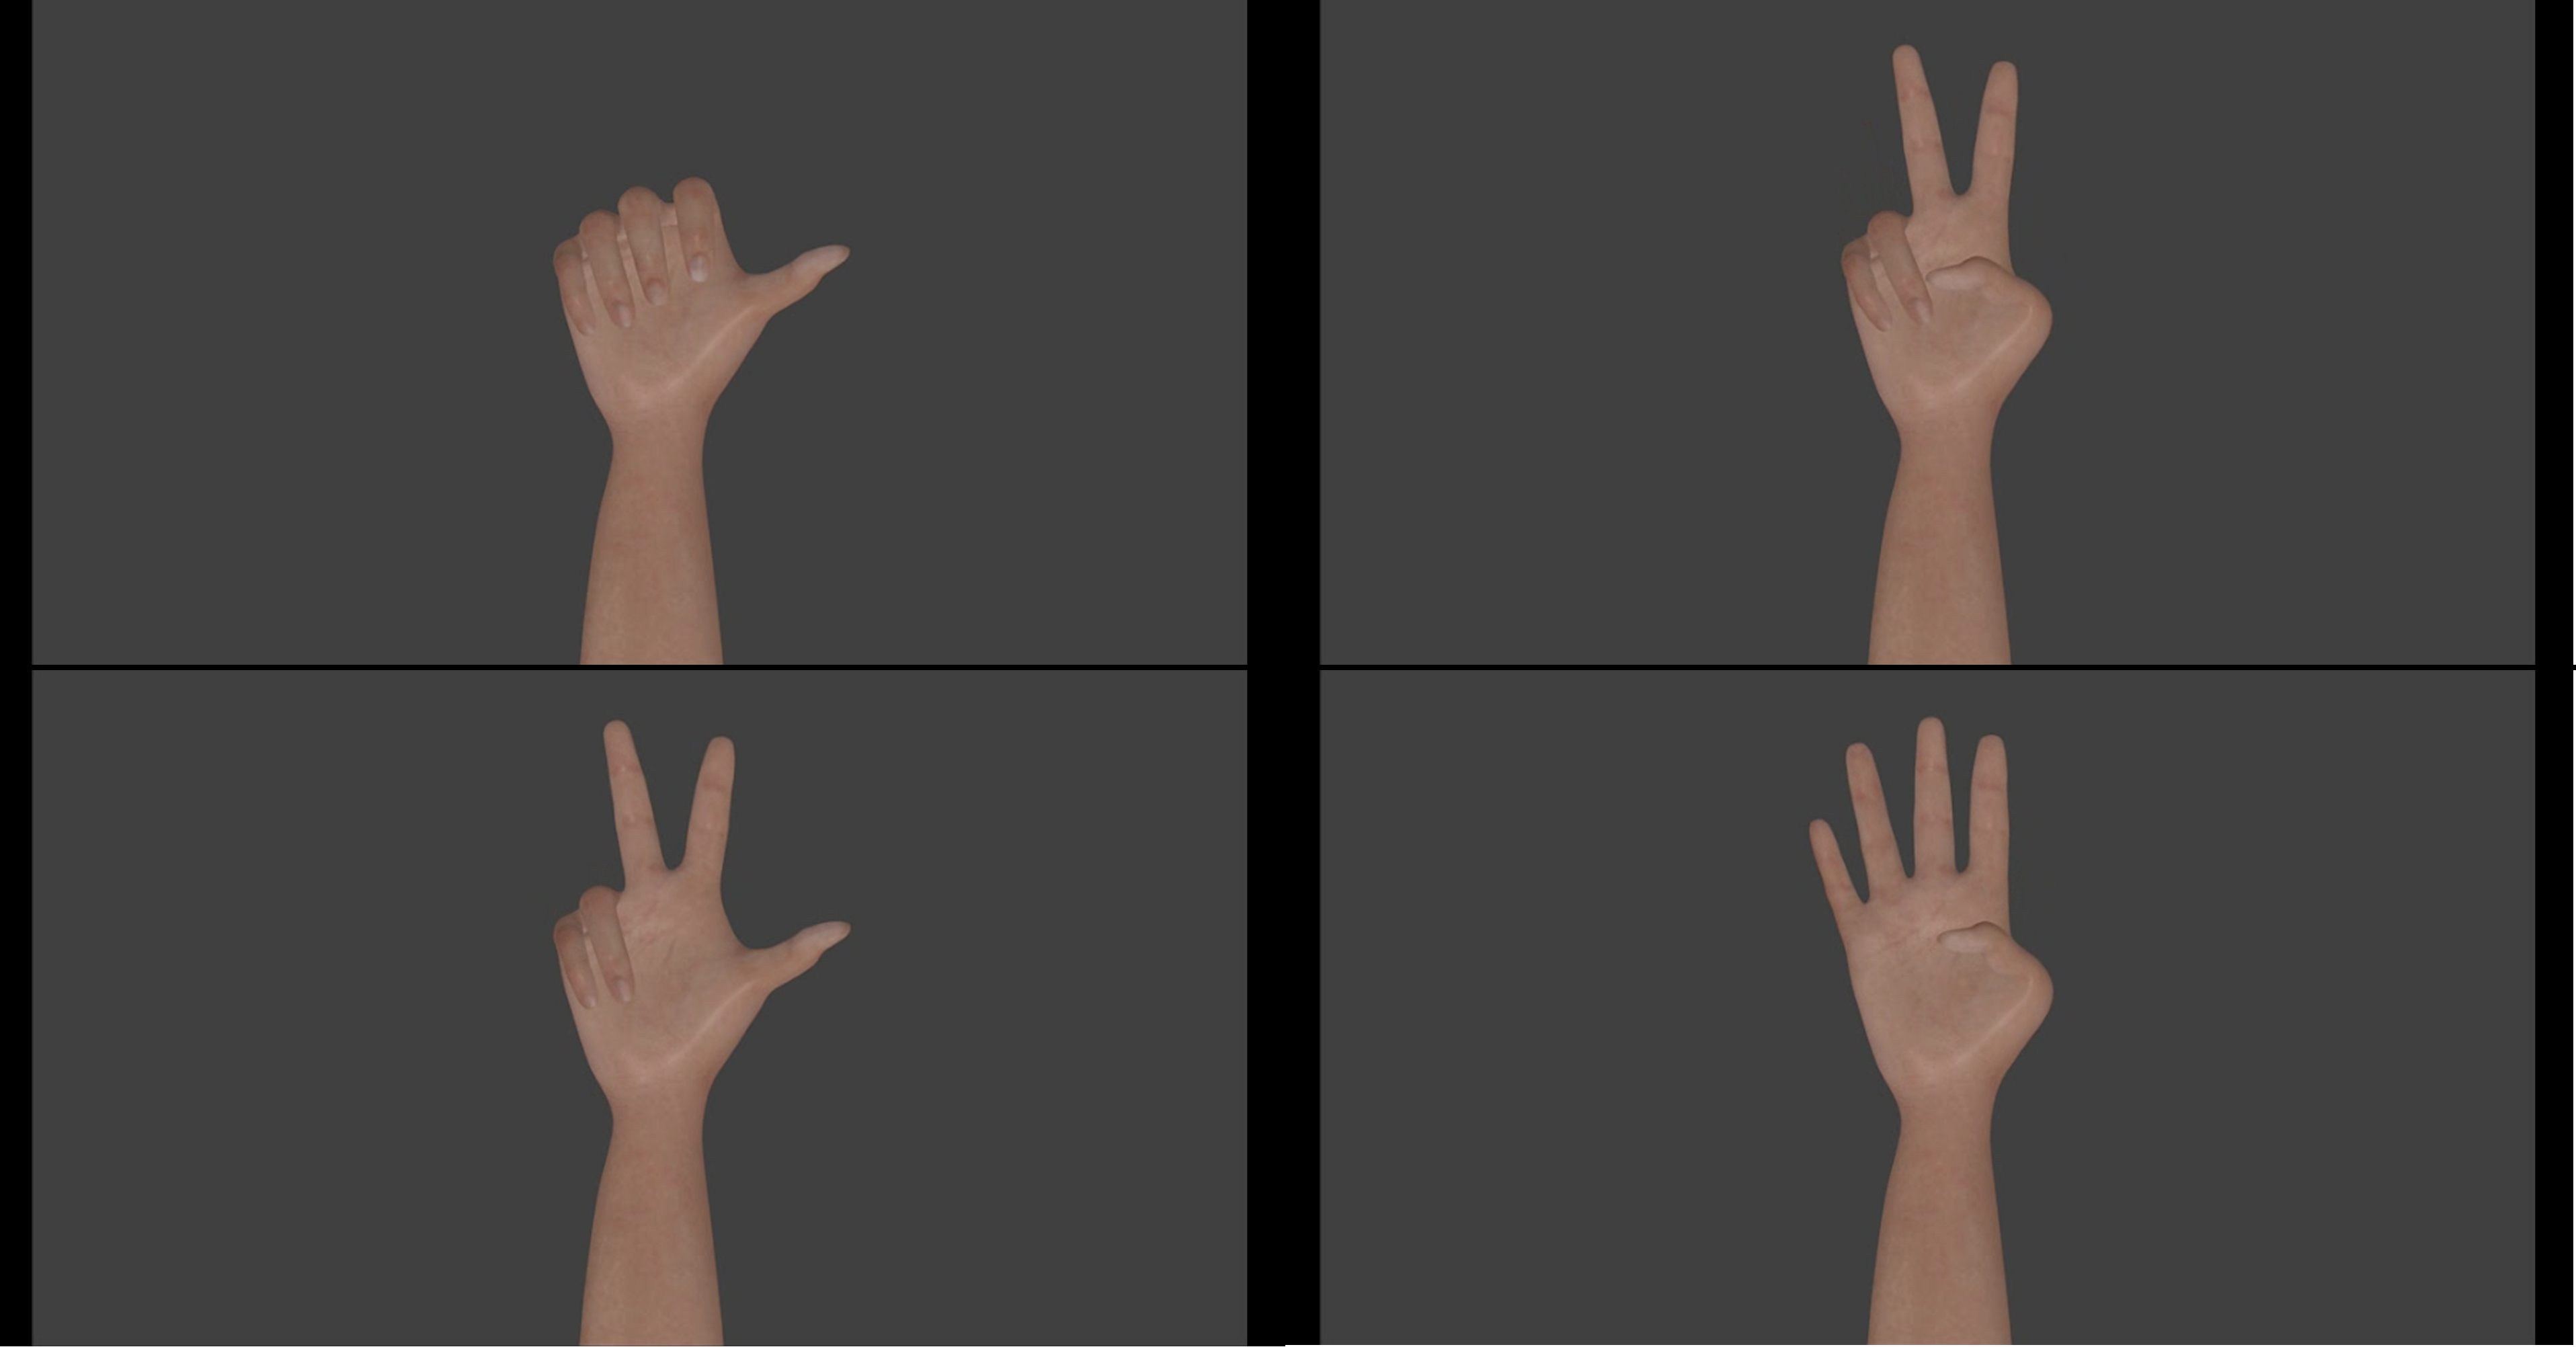
\includegraphics[width=0.75\linewidth]{./img/scenes.png}
	\end{center}
	\legend{Fonte: Laboratório de Intrumentação Eletro-Eletrônica, UFRGS}
\end{figure}

Primeiramente, realiza-se um ``treinamento'' com o voluntário, exibindo o vídeo e apresentando os movimentos que devem ser realizados (sem aquisição de sinal), de modo a reduzir possíveis erros na realização de movimentos para uma segunda exibição, quando os sinais de EMG serão devidamente adquiridos. Cada movimento apresentado em vídeo tem duração de 5 segundos, com um intervalo de 3 segundos de repouso entre movimentos. O voluntário realiza 6 repetições consecutivas para os 17 movimentos descritos na Tabela \ref{tab:movimentos}.

\begin{table}[htb]
	\begin{tabular}{m{0.5cm} m{1.5cm} m{2cm} | m{0.5cm} m{1.5cm} m{2cm} | m{0.5cm} m{1.5cm} m{2cm}}
		\toprule
		\# & Descrição & Imagem \newline demonstrativa	& \# & Descrição & Imagem \newline demonstrativa & \# & Descrição & Imagem \newline demonstrativa\\
		\midrule \midrule					
		1	&	Polegar esticado, flexão dos outros dedos.	& 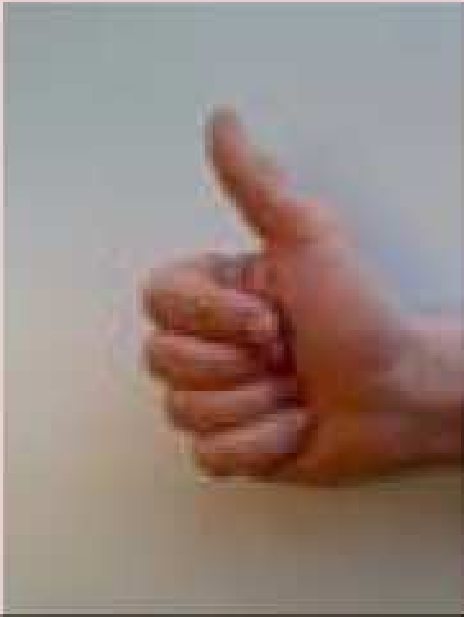
\includegraphics[width=\linewidth]{./img/moves/mov1.png} &
		2	&	Extensão do indicador e dedo médio, flexão dos outros dedos.	& 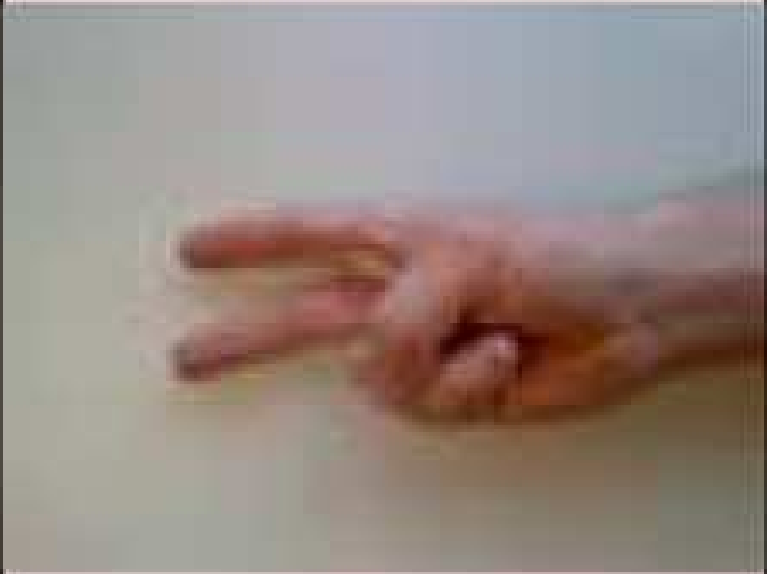
\includegraphics[width=\linewidth]{./img/moves/mov2.png} &
		3	&	Flexão do dedo anelar e mínimo, extensão dos outros dedos.	& 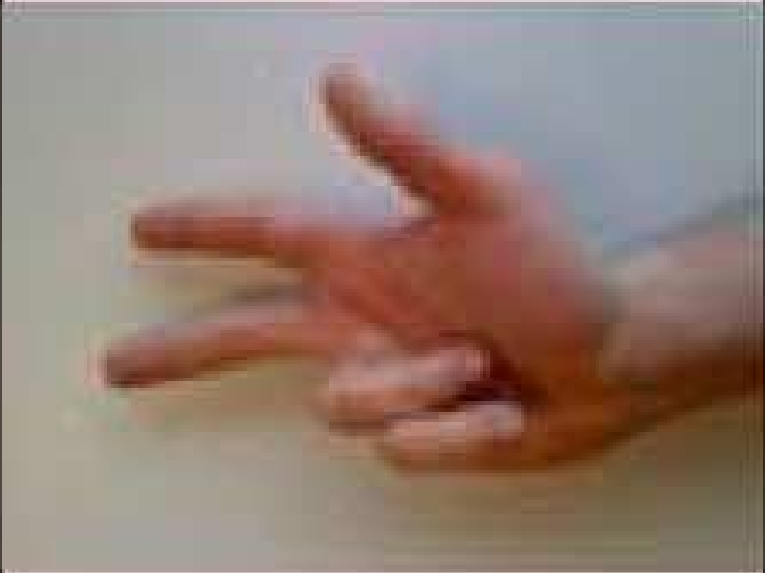
\includegraphics[width=\linewidth]{./img/moves/mov3.png}\\
		\midrule
		4	&	Polegar para a base do dedo mínimo.	& 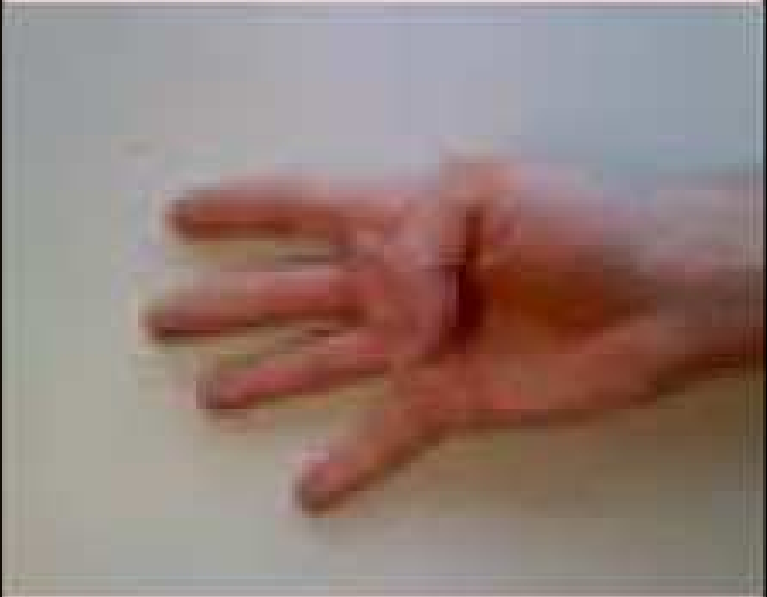
\includegraphics[width=\linewidth]{./img/moves/mov4.png} &
		5	&	Abdução (``afastamento'') de todos os dedos extendidos.	& 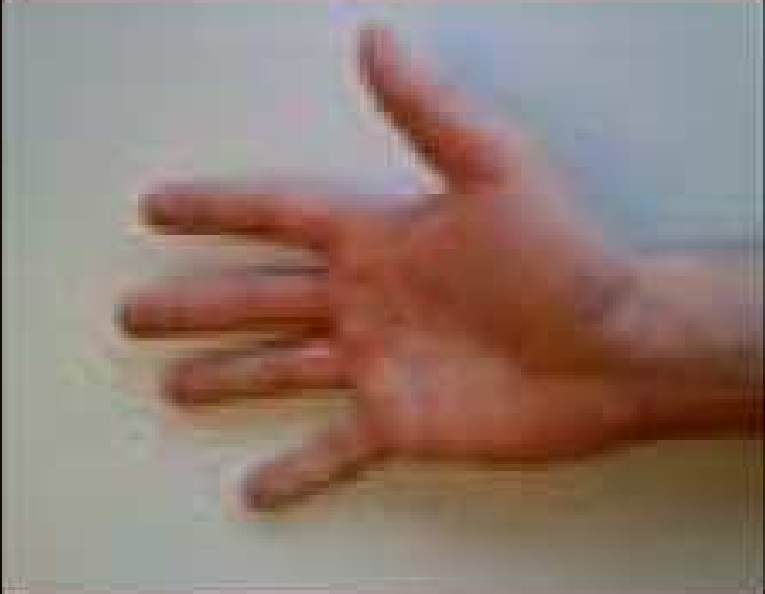
\includegraphics[width=\linewidth]{./img/moves/mov5.png} &
		6	&	Flexão de todos os dedos ao punho.	& 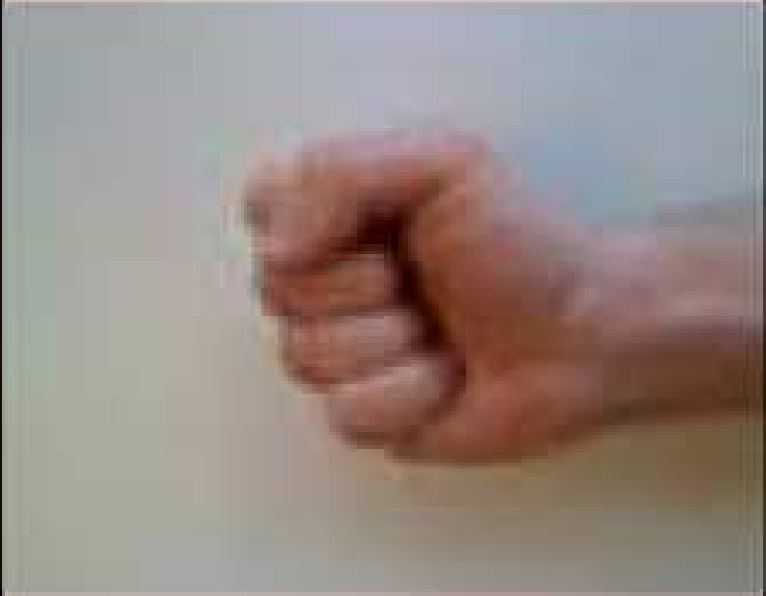
\includegraphics[width=\linewidth]{./img/moves/mov6.png}\\
		\midrule
		7	&	Extensão do indicador em movimento de ``apontar''.	& 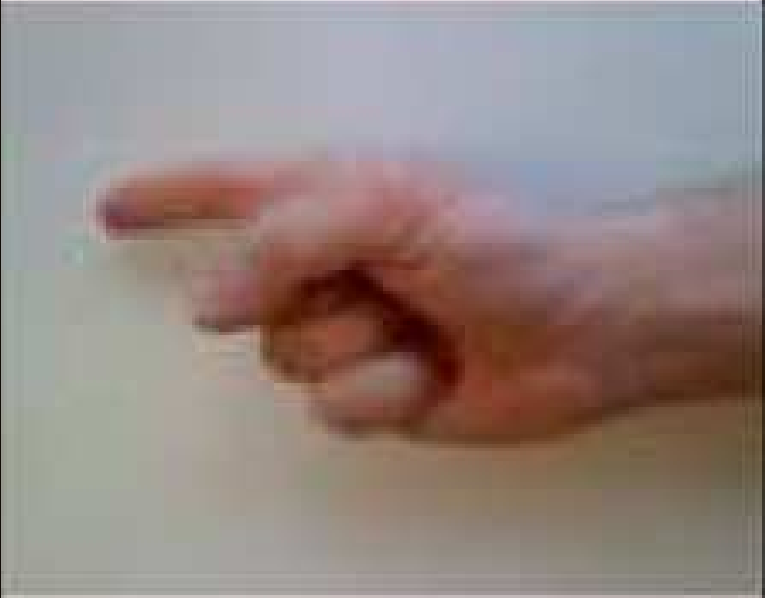
\includegraphics[width=\linewidth]{./img/moves/mov7.png} &
		8	&	Adução (``aproximação'') de todos os dedos extendidos.	& 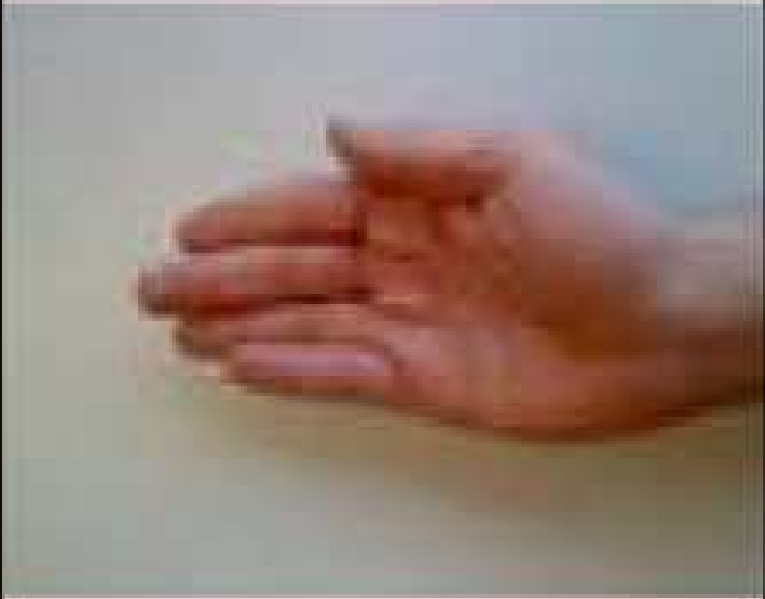
\includegraphics[width=\linewidth]{./img/moves/mov8.png} &
		9 10	&	Rotação de punho em torno do dedo médio, dois sentidos.	& 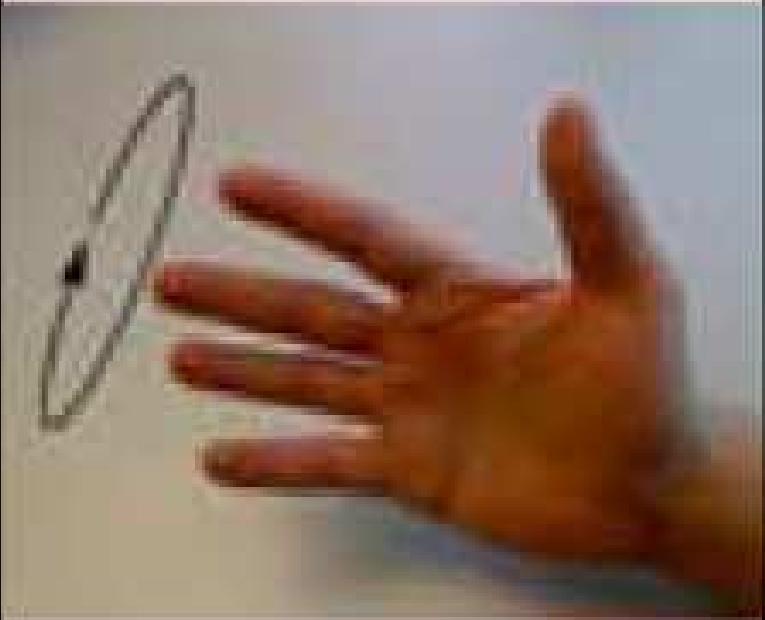
\includegraphics[width=\linewidth]{./img/moves/mov9.png} 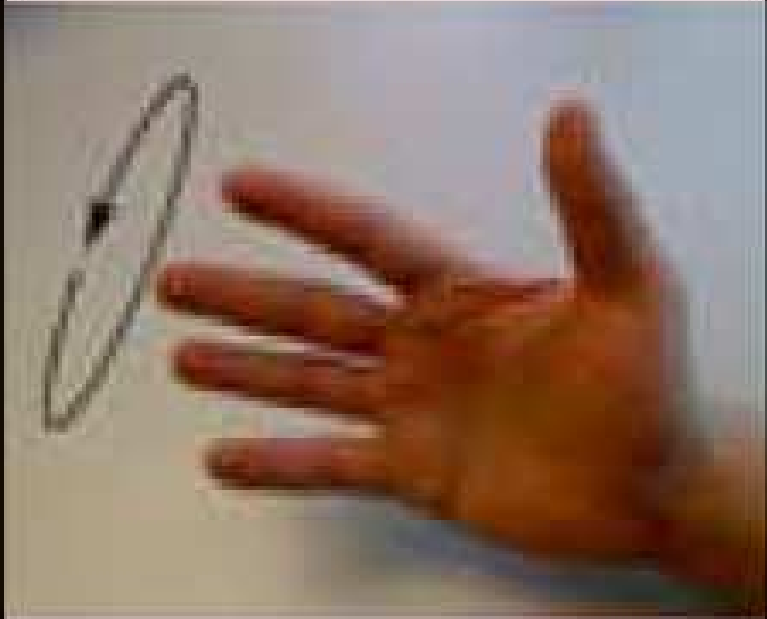
\includegraphics[width=\linewidth]{./img/moves/mov10.png} \\
		\midrule
		11 12	&	Rotação de punho em torno do dedo mínimo, dois sentidos.	& 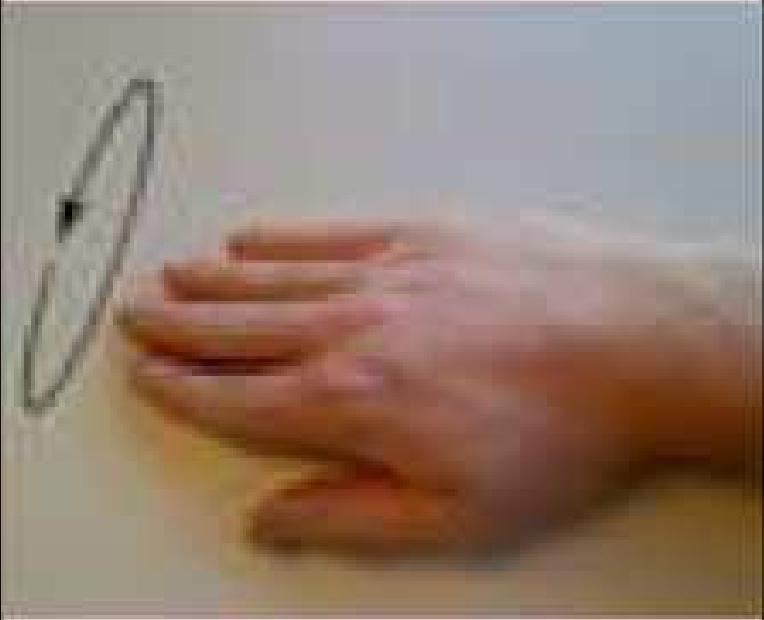
\includegraphics[width=\linewidth]{./img/moves/mov11.png} 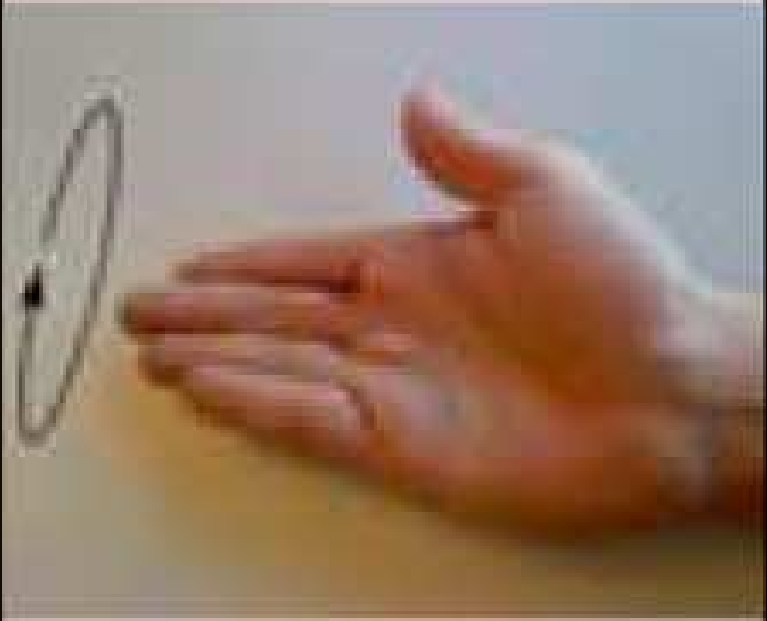
\includegraphics[width=\linewidth]{./img/moves/mov12.png} &
		13	&	Flexão de punho.	& 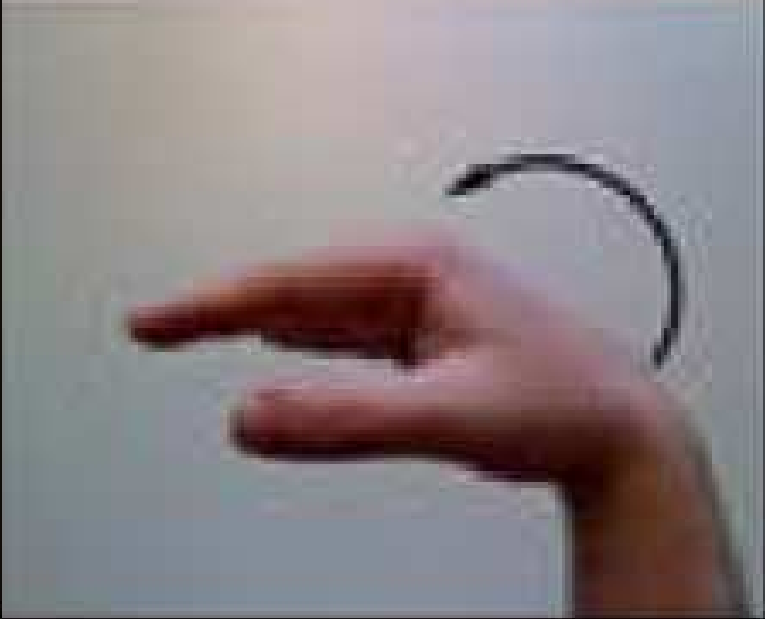
\includegraphics[width=\linewidth]{./img/moves/mov13.png} &
		14	&	Extensão de punho.	& 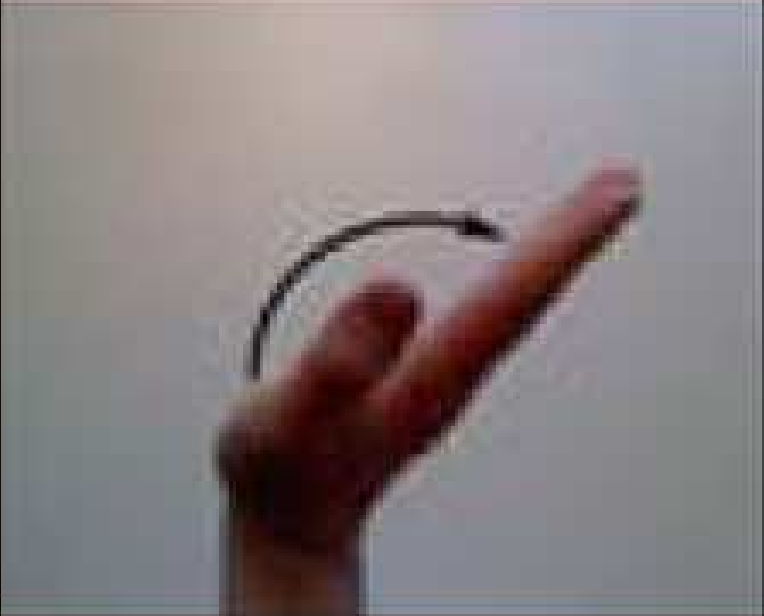
\includegraphics[width=\linewidth]{./img/moves/mov14.png}\\
		\midrule
		15	&	Desvio radial do punho.	& 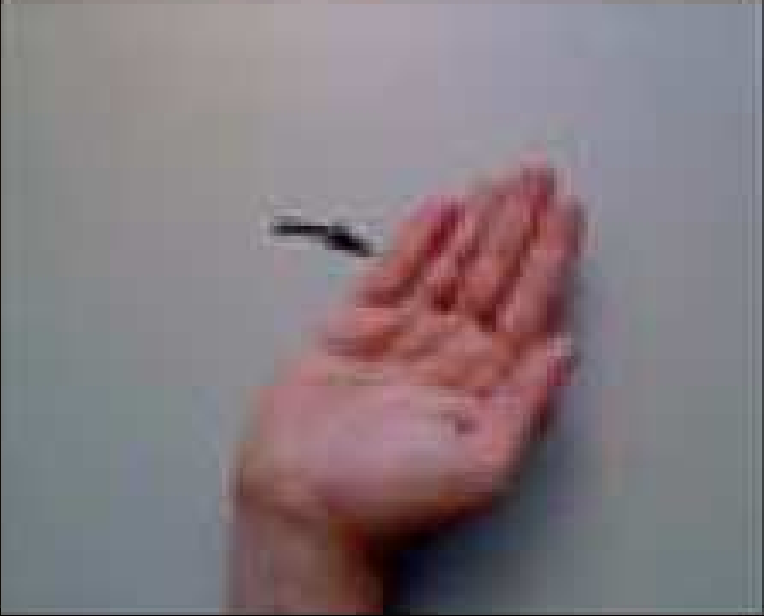
\includegraphics[width=\linewidth]{./img/moves/mov15.png} &
		16	&	Desvio ulnar do punho.	& 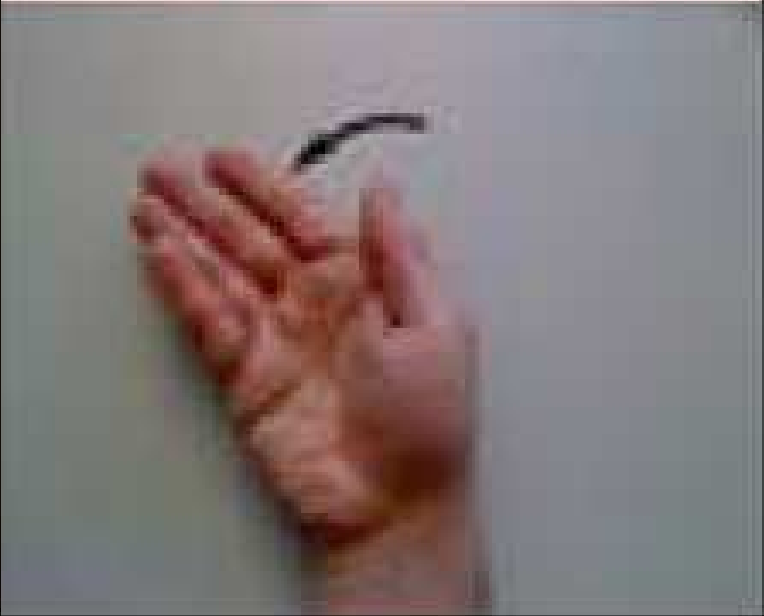
\includegraphics[width=\linewidth]{./img/moves/mov16.png} &
		17	&	Extensão de punho com mão cerrada.	& 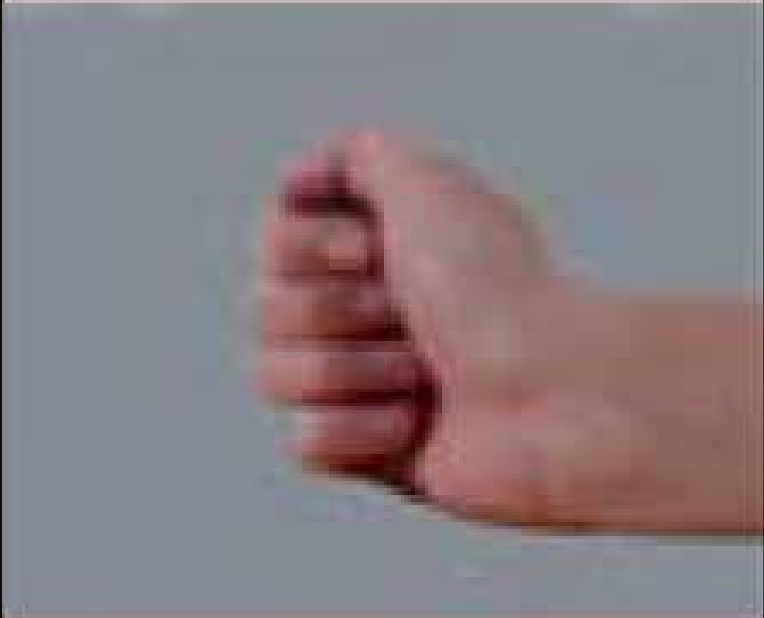
\includegraphics[width=\linewidth]{./img/moves/mov17.png}\\
		\bottomrule
	\end{tabular}
\end{table}


%=========================================================================
		\section{Métodos de Segmentação}
%=========================================================================
Esta seção descreve a implementação dos métodos de segmentação propostos. O diagrama de blocos da Figura \ref{flow:MTDs} apresenta de forma resumida os passos comuns aos quatro métodos, que serão explanados nas subseções seguintes. Os códigos criados para os quatro métodos, escritos para MATLAB R2015a, encontram-se nos Apêndices \ref{ap:seg_mtd1} a \ref{ap:seg_mtd4}.

% Set up a few colours
\colorlet{lcfree}{green}
\colorlet{lcnorm}{blue}
\colorlet{lccong}{red}
% -------------------------------------------------
% Set up a new layer for the debugging marks, and make sure it is on
% top
\pgfdeclarelayer{marx}
\pgfsetlayers{main,marx}
% A macro for marking coordinates (specific to the coordinate naming
% scheme used here). Swap the following 2 definitions to deactivate
% marks.
\providecommand{\cmark}[2][]{%
  \begin{pgfonlayer}{marx}
    \node [nmark] at (c#2#1) {#2};
  \end{pgfonlayer}{marx}
  } 
\providecommand{\cmark}[2][]{\relax} 
% -------------------------------------------------
% Start the picture
\begin{figure}[htb]
	\caption{\label{flow:MTDs} Diagrama de blocos geral para os métodos de segmentação MTD1 - MTD4.}
	\begin{center}
		\begin{tikzpicture}[%
			>=triangle 60,              % Nice arrows; your taste may be different
			start chain=going below,    % General flow is top-to-bottom
			node distance=6mm and 60mm, % Global setup of box spacing
			every join/.style={norm},   % Default linetype for connecting boxes
			]
		% ------------------------------------------------- 
		% A few box styles 
		% <on chain> *and* <on grid> reduce the need for manual relative
		% positioning of nodes
		\tikzset{
		  base/.style={draw, on chain, on grid, align=center, minimum height=4ex},
		  proc/.style={base, rectangle, text width=8em},
		  test/.style={base, diamond, aspect=2, text width=8em},
		  term/.style={proc, rounded corners},
		  % coord node style is used for placing corners of connecting lines
		  coord/.style={coordinate, on chain, on grid, node distance=6mm and 25mm},
		  % nmark node style is used for coordinate debugging marks
		  nmark/.style={draw, cyan, circle, font={\sffamily\bfseries}},
		  % -------------------------------------------------
		  % Connector line styles for different parts of the diagram
		  norm/.style={->, draw, lcnorm},
		  free/.style={->, draw, lcfree},
		  cong/.style={->, draw, lccong},
		  it/.style={font={\small\itshape}}
		}
		% -------------------------------------------------
		% Node placement: column 1
		\node [proc, fill=lcfree!25] (pre) {Preprocessamento (retificação e normalização)};
		\node [proc, fill=lcfree!25, right=of pre, xshift=-4em, join] (id) {Identificação de segmentos para cada canal utilizando MTD\#};
		\node [proc, fill=lcfree!25, right=of id, xshift=-4em, join] (dbscan) {Agrupamento de posições de segmentos utilizando DBSCAN};
		\node [proc, fill=lcfree!25, right=of dbscan, xshift=-4em, join] {Segmentação do sinal nas médias das posições agrupadas};
		% -------------------------------------------------
		\end{tikzpicture}
	\end{center}
\end{figure}


%-------------------------------------------------------------------------
			\subsection {Preprocessamento}
%-------------------------------------------------------------------------

Os sinais de eletromiografia para ambas as bases de dados (NinaPro e IEE) são armazenados mantendo sua polaridade original (i.e. amostras do sinal podem assumir valores positivos e negativos). Primeiramente, realiza-se a retificação completa dos sinais tomando o módulo dos valores amostrados (em MATLAB, função \emph{abs()}). A retificação completa do sinal mantém sua energia e é fundamental para a implementação dos métodos de segmentação aqui desenvolvidos.

Após a etapa de retificação, os sinais para cada canal de aquisição são normalizados de acordo com seu valor máximo, de modo que seu novo valor máximo seja unitário, a partir da Equação (\ref{eq:x_normalization}), onde $x$ é o sinal original para um canal e $x_{norm}$ é sua versão normalizada. A normalização de canais faz com que os parâmetros utilizados pelos métodos de segmentação sejam relativos ao valor máximo do sinal, possibilitando a implementação para diferentes voluntários. A Figura \ref{fig:normalization} exemplifica retificação e normalização para trecho de sinal de um canal de EMG.

\begin{equation}
	\label{eq:x_normalization}
	x_{norm} = \frac{x}{max(x)}
\end{equation}

\begin{figure}[htb]
	\caption{\label{fig:normalization}Exemplo para retificação e normalização de trecho de sinal de EMG.}
	\begin{center}
	    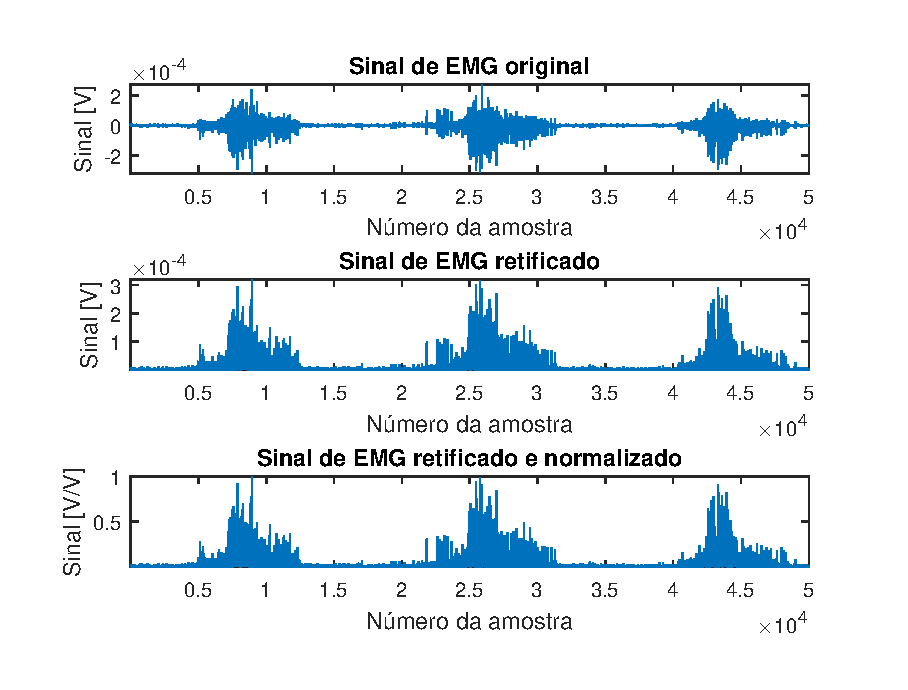
\includegraphics[width=0.75\linewidth]{./img/matlab/prettyRaw.eps}
	\end{center}
	%\legend{Fonte: adaptado de BASMAJIAN \& DE LUCA, 1985}
\end{figure}

%-------------------------------------------------------------------------
				\subsection{Parâmetros Ajustáveis}
%-------------------------------------------------------------------------
Cada método de segmentação MTD1 - MTD4 apresenta um conjunto de parâmetros ajustáveis. Tais parâmetros foram descritos anteriormentes na Seção \ref{sec:MTDs} (Tabelas \ref{tab:mtd1params} a \ref{tab:mtd4params}). Após investigações iniciais de segmentações obtidas com diferentes valores de parâmetros, listou-se valores a serem explorados na aplicação de cada método. A Tabela \ref{tab:combinacoes} apresenta os parâmetros ajustáveis de cada método e sua respectiva lista de valores explorados.

\begin{table}[htb]
\IBGEtab{\caption{\label{tab:combinacoes}Parâmetros ajustáveis para os métodos de segmentação.}}
{
	\begin{tabular}{cllc}
		\toprule
		Método 					& Parâmetros	& Valores utilizados						& Número total de combinações \\
		\midrule \midrule					
		\multirow{4}{*}{MTD1}	& $l$			& $10 \times 10^3$							& \multirow{4}{*}{16} \\
								& $r_{target}$	& $5,6 \times 10^{-5}$						& \\
								& $q$			& $[0.8 \quad 0.85 \quad 0.9 \quad 0.95]$	& \\
								& $T_{lim`}$	& $[0.05 \quad 0.1 \quad 0.15 \quad 0.2]$	& \\
		\midrule
		\multirow{4}{*}{MTD2}	& $l$			& $10 \times 10^3$							& \multirow{4}{*}{27} \\
								& $A$			& $[20 \quad 30 \quad 40]$					& \\
								& $B$			& $[2 \quad 5 \quad 8]$						& \\
								& $C$			& $[2 \quad 5 \quad 8]$						& \\
		\midrule					
		\multirow{3}{*}{MTD3}	& $W$			& TODO										& \multirow{3}{*}{TODO} \\
								& $B$			& TODO										& \\
								& $C$			& TODO										& \\
		\midrule					
		\multirow{2}{*}{MTD4}	& $W$			& TODO										& \multirow{2}{*}{TODO} \\
								& $T$			& TODO										& \\
		\bottomrule
	\end{tabular}
}{}
\end{table}


Para os métodos que necessitam parâmetro de comprimento de segmento $l$ (i.e. os métodos que produzem segmentos de comprimento de janela constante, MTD1 e MTD2) utilizou-se valor de $l$ como $10 \times 10^3$, que corresponde a 5 cinco segundos de aquisição para ambas as bases de dados (período de amostragem para ambas é de 500 $\mu s$), sendo a mesma duração dos segmentos de vídeo replicados pelos voluntários.

Para os métodos que utilizam janela deslizante (MTD3 e MTD4), utilizou-se comprimento de janela $W$ de 5000 amostras, de modo que o comprimento temporal da janela (2,5 segundos) equivale à metade da duração do segmento de vídeo, com incrementos $step$ de 100 amostras. Os parâmetros de $l_{mín}$ e $l_{máx}$ utilizados foram de 7500 e 12500 amostras, respectivamente.

O valor de $r_{target}$  para o MTD1 foi obtido utilizando o código do Apêndice \ref{ap:r_target} como sendo valor mínimo da razão entre número de segmentos e comprimento de sinal para os voluntários de cada base de dados da NinaPro e IEE.

%-------------------------------------------------------------------------
			\subsection{Agrupamento das Posições de Segmentos de Diferentes Canais Utilizando DBSCAN}
%-------------------------------------------------------------------------
Como já mencionado, os sinais para ambas as bases de dados são compostos por doze canais de aquisição. Os métodos de segmentação são implementados individualmente para os doze canais. Para os métodos MTD1 e MTD2, posições centrais dos segmentos obtidas em cada canal são armazenadas, enquanto que para os métodos MTD3 e MT4 armazena-se as posições de BEPs e EEPs. Tais posições de diferentes canais são identificadas como pertencendo a um mesmo segmento através do algoritmo de grupamento DBSCAN (\emph{Density-Based Spatial Clustering of Applications with Noise}).

DBSCAN foi inicialmente proposto em \cite{Ester1996} para grupamento de pontos utilizando dois parâmetros: $\epsilon$, que define uma vizinhança em torno do valor de cada ponto, e $minPts$, que determina o número mínimo de pontos pertencentes à mesma vizinhança para formação do ``núcleo'' de um grupo. Para mais detalhes sobre DBSCAN, sugere-se o artigo original \cite{Ester1996} e a revisão do método \cite{Thanh2013}, cujo código em MATLAB foi utilizado (Apêndice \ref{ap:dbscan}). 

Na implementação dos quatro métodos, utilizou-se $\epsilon = 2000$ amostras e $minPts = 3$ canais. Em outras palavras, isto significa que para a identificação de um centro de segmento (métodos MTD1 e MTD2) ou de BEPs e EEPs (métodos MTD3 e MTD4) é necessário que as posições identificadas, em pelo menos 3 diferentes canais, pertençam a uma vizinhança bilateral de 4000 amostras (2 segundos de aquisição).

O algoritmo DBSCAN foi escolhido para esta aplicação por dois motivos principais. Primeiramente, ao contrário de métodos de grupamento como \emph{k-means}, DBSCAN não necessita parâmetro que especifique número de grupos, no caso, número de segmentos a serem obtidos, o que mantém o caráter ``automático'' dos métodos de segmentação. Além disto, o parâmetro $minPts$ faz com que este método seja capaz de descartar posições \emph{outliers} que venham a ser identificadas por canal. Sendo assim, o algoritmo DBSCAN é capaz de tornar mais robusto os métodos de segmentação e implementáveis a sinais de múltiplos canais.

Após o agrupamento de posições de segmentos obtidos nos diferentes canais, tomam-se as médias de cada grupo como as posições nas quais o sinal deve ser segmentado (para os métodos MTD1 e MTD2, as médias dos grupos indicam posições centrais de segmentos e para métodos MTD3 e MTD4 indicam posições de BEPs e EEPs). O sinal é segmentado nestas posições para os doze canais, mantendo a coerência temporal entre canais.

%=========================================================================
		\section{Classificação de Segmentos com Redes Neurais Artificiais}
%=========================================================================
Esta seção descreve o uso de RNAs para classificação dos segmentos obtidos de acordo com movimentos de interesse. O processo de classificação é representado pelo diagrama de blocos da Figura \ref{flow:RNAs}, que será explanado nas subseções seguintes.

% Set up a few colours
\colorlet{lcfree}{green}
\colorlet{lcnorm}{blue}
\colorlet{lccong}{red}
% -------------------------------------------------
% Set up a new layer for the debugging marks, and make sure it is on
% top
\pgfdeclarelayer{marx}
\pgfsetlayers{main,marx}
% A macro for marking coordinates (specific to the coordinate naming
% scheme used here). Swap the following 2 definitions to deactivate
% marks.
\providecommand{\cmark}[2][]{%
  \begin{pgfonlayer}{marx}
    \node [nmark] at (c#2#1) {#2};
  \end{pgfonlayer}{marx}
  } 
\providecommand{\cmark}[2][]{\relax} 
% -------------------------------------------------
% Start the picture
\begin{figure}[htb]
	\caption{\label{flow:RNAs} Fluxograma da classificação de movimentos com RNAs.}
	\begin{center}
		\begin{tikzpicture}[%
			>=triangle 60,              % Nice arrows; your taste may be different
			start chain=going below,    % General flow is top-to-bottom
			node distance=6mm and 60mm, % Global setup of box spacing
			every join/.style={norm},   % Default linetype for connecting boxes
			]
		% ------------------------------------------------- 
		% A few box styles 
		% <on chain> *and* <on grid> reduce the need for manual relative
		% positioning of nodes
		\tikzset{
		  base/.style={draw, on chain, on grid, align=center, minimum height=4ex},
		  proc/.style={base, rectangle, text width=8em},
		  test/.style={base, diamond, aspect=2, text width=8em},
		  term/.style={proc, rounded corners},
		  % coord node style is used for placing corners of connecting lines
		  coord/.style={coordinate, on chain, on grid, node distance=6mm and 25mm},
		  % nmark node style is used for coordinate debugging marks
		  nmark/.style={draw, cyan, circle, font={\sffamily\bfseries}},
		  % -------------------------------------------------
		  % Connector line styles for different parts of the diagram
		  norm/.style={->, draw, lcnorm},
		  free/.style={->, draw, lcfree},
		  cong/.style={->, draw, lccong},
		  it/.style={font={\small\itshape}}
		}
		% -------------------------------------------------
		% Node placement: column 1
		\node [term, densely dotted, it, fill=lccong!25] (init) {INÍCIO};
		\node [proc, fill=lcfree!25, right=of init, xshift=-4em, join] (pre) {Segmentar o sinal com o MTD\#};
		\node [proc, fill=lcfree!25, right=of pre, xshift=-4em, join] (id) {Identificação de movimento associado a cada segmento (vetor de respostas)};
		\node [proc, fill=lcfree!25, right=of id, xshift=-4em, join] (dbscan) {Extração de características dos segmentos};
		\node [proc, fill=lcfree!25, join] (sep) {Separação de segmentos em grupos para treino, validação e teste};
		\node [proc, fill=lcfree!25, join, left=of sep, xshift=2em] (train) {Treinamento da RNA};
		\node [proc, fill=lcfree!25, join, left=of train, xshift=2em] {Obtenção de resultados de para todos os segmentos};
		% -------------------------------------------------
		\end{tikzpicture}
	\end{center}
\end{figure}


%-------------------------------------------------------------------------
			\subsection{Características Utilizadas como Preditores}
%-------------------------------------------------------------------------
Os preditores (``entradas'') das RNAs são o valor RMS, a variância e a frequência mediana do espectro de potência dos segmentos de sinal obtidos pelos métodos MTD1 - MTD4. Tais características foram selecionados de acordo com outros trabalhos já realizados no Laboratório de Instrumentação Eletro-Eletrônica que obtiveram bons resultados em métodos de inteligência computacional, como \cite{Favieiro2009}, \cite{Schons2014} e \cite{Cene2015}.

O valor RMS ou \emph{Root Mean Square} de um sinal discreto \emph{x} de comprimento $L$ (em MATLAB, função \emph{rms()}) é dada pela Equação (\ref{eq:rms}) e a variância deste sinal (em MATLAB, função \emph{var()}) é dada pela Equação (\ref{eq:var}), onde $\bar{x}$ é o valor médio do sinal. A frequência mediana é tal que a soma total da densidade de potência para frequências abaixo da frequência mediana é igual à soma total da densidade de potência para frequências acima da frequência mediana, sendo estimada pela função \emph{medfreq()} em MATLAB.

\begin{equation}
	\label{eq:rms}
	rms(x) = \sqrt{\frac{1}{L}\sum\limits_{i=1}^{L}x_i^2} 
\end{equation}

\begin{equation}
	\label{eq:var}
	var(x) = \frac{1}{L-1}\sum\limits_{i=1}^{L}(x_i - \bar{x})^2
\end{equation}

%-------------------------------------------------------------------------
			\subsection{Classes de Movimentos Utilizadas como Resposta}
%-------------------------------------------------------------------------
Realiza-se a identificação de movimentos associados a cada segmento obtido a partir de sua posição temporal no sinal original, já que em ambas as bases de dados os movimentos são realizados na mesma sequência para todos os voluntários.

A base de dados NinaPro contém um \emph{array stimulus} que indica os instantes em que foi exibida em vídeo cada classe de movimentos a serem replicados pelo voluntário. Este \emph{array} é utilizado para obter a relação entre posições de segmentos e classes de movimentos.

A base de dados IEE não contém tal \emph{array}. A classe de movimento associada ao segmento é identificada a partir da posição do segmento relativa ao comprimento total do sinal - considera-se que cada décima-sétima parte do comprimento total do sinal corresponde a uma classe de movimentos distina.

A função apresentada no Apêndice \ref{ap:idMoves} é utilizada para criar o vetor de respostas esperadas no treinamento da RNA, tendo como argumentos as posições centrais de segmentos (para os métodos MTD3 e MTD4, calcula-se média dos pares BEP-EEP), uma \emph{string} identificadora da base de dados utilizada e, dependendo da base utilizada, \emph{array stimulus} ou o comprimento total do sinal $L$.

%-------------------------------------------------------------------------
			\subsection{Separação de Grupos de Treino, Validação e Teste para Treinamento}
%-------------------------------------------------------------------------
Sendo $N_i$ o número de segmentos obtidos por classe de movimentos $i$, os grupos de segmentos utilizados nos treinamentos de RNAs são tais que: 

\begin{itemize}
\item grupo de treino: primeiros $N_i-2$ segmentos obtidos de todas as classes de movimentos
\item grupo de validação: segmento obtido de índice $N_i-1$ de todas as classes de movimentos
\item grupo de teste: $N_i$-ésimo segmento obtido de todas as classes de movimentos
\item Para $N_i=2$, o primeiro segmento identificado da classe $i$ entra no grupo de treino e o segundo segmento no grupo de validação.
\item Para $N_i=1$, o segmento identificado da classe $i$ entra no grupo de treino.
\end{itemize}

Optou-se por este controle da divisão por indexação (método de divisão chamado em MATLAB de $divideind$) ao invés de métodos de divisão aleatória de grupos ($dividerand$) devido ao número reduzido de repetições por classe de movimento (6 repetições). Utilizar divisão aleatória de grupos apresentaria alta chance de situações particulares em que nenhum (ou, na situação oposta e igualmente indesejada, todos) segmentos de determinada classe estariam inclusos no grupo ``treino'', viciando resultados de classificação.

%-------------------------------------------------------------------------
			\subsection{Estrutura de RNAs Treinadas}
%-------------------------------------------------------------------------
As RNAs utilizadas para todos os métodos são do tipo \emph{feedforward}, compostas por uma camada oculta e uma camada de saída, sendo a camada oculta formada por 40 neurônios com função de ativação $logsig()$ (Equação (\ref{eq:logsig})) e a camada de saída por 17 neurônios, um para cada classe de movimento, sendo que nesta camada o neurônio com saída de maior valor indica qual a classe de movimento em que foi classificado o segmento.

A Figura \ref{fig:matlabRNA} mostra a representação esquemática realizada pelo MATLAB para a estrutura das RNAs. O bloco \emph{Input} (``entrada'') indica o uso total de 36 preditores, referentes a segmentos de sinal com 12 canais e 3 preditores por canal (RMS, variância e frequência mediana). Na camada \emph{Hidden} (``oculta'') indica-se o uso de 40 neurônios com função de ativação $logsig()$ e a camada \emph{Output} (``saída'') representa os 17 neurônios que indicam resultados de classificação.

\begin{figure}[htb]
	\caption{\label{fig:matlabRNA}Estrutura de RNAs utilizadas.}
	\begin{center}
	    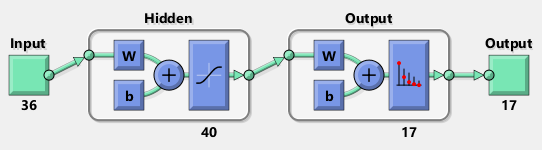
\includegraphics[width=0.75\linewidth]{./img/matlabRNA.png}
	\end{center}
	%\legend{Fonte: adaptado de BASMAJIAN \& DE LUCA, 1985}
\end{figure}


%=========================================================================
% RESULTADOS E DISCUSSÕES
	\chapter{Resultados e Discussões}
%=========================================================================
		\section{Número de Segmentos por Classe de Movimentos Obtidos com os Métodos MTD1 a MTD4 e Valor $F$ em Diferentes Combinações de Parâmetros}
%-------------------------------------------------------------------------
As diferentes combinações de parâmetros testadas nos métodos MTD1 a MTD4 foram indexadas por método de segmentação de acordo com a Tabela \ref{tab:combinacoes_expanded}. As Figuras \ref{fig:mtd1Nina} a \ref{fig:mtd4Iee} apresentam resultados de média e moda de número de segmentos obtidos por classe de movimento com a implementação de cada combinação de parâmetros dos métodos a todos os voluntários de cada base de dados. Também apresenta-se resultados para valor $F$ médio entre todos as classes de movimentos e todos os voluntários de uma mesma base de dados.

\begin{table}[htb]
\IBGEtab{\caption{\label{tab:combinacoes_expanded}Combinações de parâmetros utilizados nos métodos de segmentação.}}
{
	\begin{tabular}{cc|cc|ccc|cc|c}
		\toprule
		\multicolumn{2}{c}{Método\#} & \multicolumn{2}{c}{1} & \multicolumn{3}{c}{2} & \multicolumn{2}{c}{3} & 4\\
		\midrule
		\multicolumn{2}{c}{Parâmetro}	&q&$T_{lim}$&A&B&C&B&C&T \\
		\midrule \midrule					
		\multirow{27}{*}{\rotatebox{90}{Índice da Combinação}} &
		1 &0.80&0.05&&&&&\\
		&2 &0.85&0.05&&&&&\\
		&3 &0.90&0.05&&&&&\\
		&4 &0.95&0.05&&&&&\\
		&5 &0.80&0.10&&&&&\\
		&6 &0.85&0.10&&&&&\\
		&7 &0.90&0.10&&&&&\\
		&8 &0.95&0.10&&&&&\\
		&9 &0.80&0.15&&&&&\\
		&10&0.85&0.15&&&&&\\
		&11&0.90&0.15&&&&&\\
		&12&0.95&0.15&&&&&\\
		&13&0.80&0.20&&&&&\\
		&14&0.85&0.20&&&&&\\
		&15&0.90&0.20&&&&&\\
		&16&0.95&0.20&&&&&\\
		&17&\-  &\-  &&&&&\\
		&18&\-  &\-  &&&&&\\
		&19&\-  &\-  &&&&&\\
		&20&\-  &\-  &&&&&\\
		&21&\-  &\-  &&&&&\\
		&22&\-  &\-  &&&&&\\
		&23&\-  &\-  &&&&&\\
		&24&\-  &\-  &&&&&\\
		&25&\-  &\-  &&&&&\\
		&26&\-  &\-  &&&&&\\
		&27&\-  &\-  &&&&&\\
		\bottomrule
	\end{tabular}
}{}
\end{table}


\begin{figure}[htb]
	\caption{\label{fig:mtd1Nina}Média e moda do número de segmentos obtidos por classe de movimento e valor $F$ médio de RNAs. Método de segmentação: MTD1. Base de dados: NinaPro}.
	\begin{center}
	    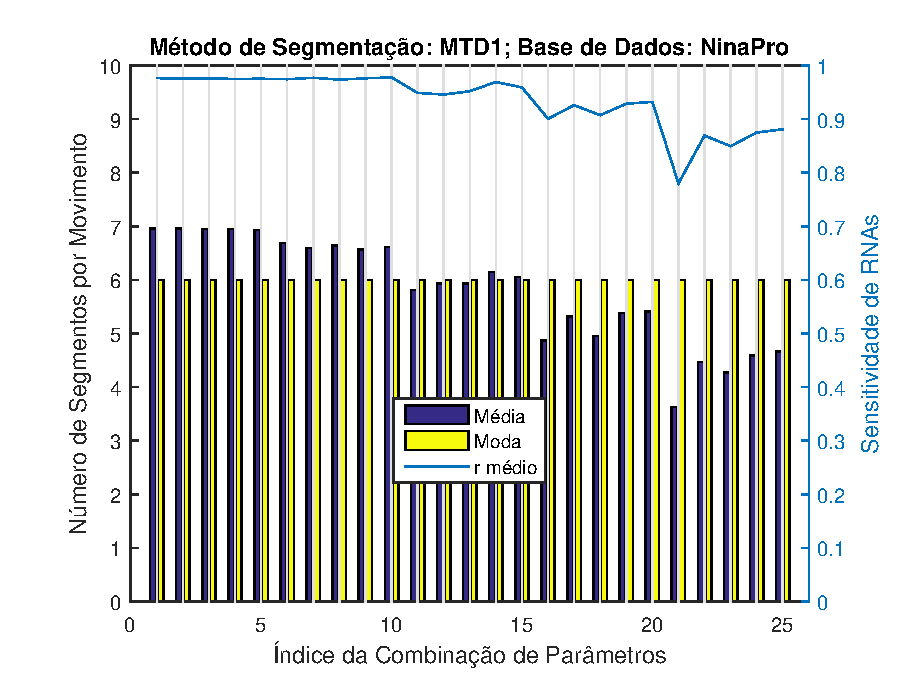
\includegraphics[width=0.75\linewidth]{./img/matlab/results/mtd1_nina.eps}
	\end{center}
	%\legend{Fonte: adaptado de BASMAJIAN \& DE LUCA, 1985}
\end{figure}

\begin{figure}[htb]
	\caption{\label{fig:mtd1Iee}Média e moda do número de segmentos obtidos por classe de movimento e valor $F$ médio de RNAs. Método de segmentação: MTD1. Base de dados: IEE}.
	\begin{center}
	    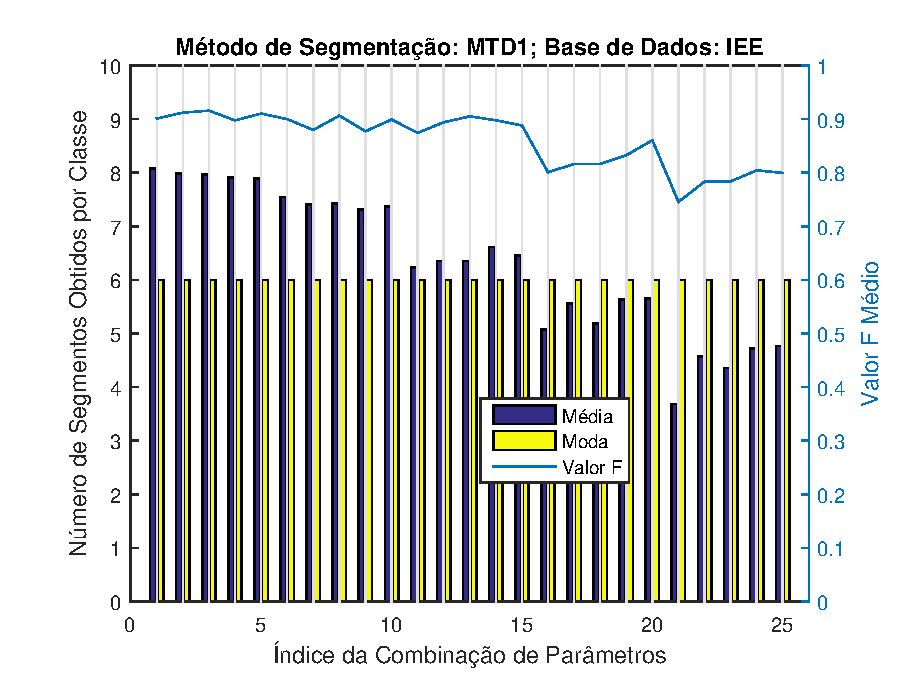
\includegraphics[width=0.75\linewidth]{./img/matlab/results/mtd1_iee.eps}
	\end{center}
	%\legend{Fonte: adaptado de BASMAJIAN \& DE LUCA, 1985}
\end{figure}

\begin{figure}[htb]
	\caption{\label{fig:mtd2Nina}Média e moda do número de segmentos obtidos por classe de movimento e valor $F$ médio de RNAs. Método de segmentação: MTD2. Base de dados: NinaPro}.
	\begin{center}
	    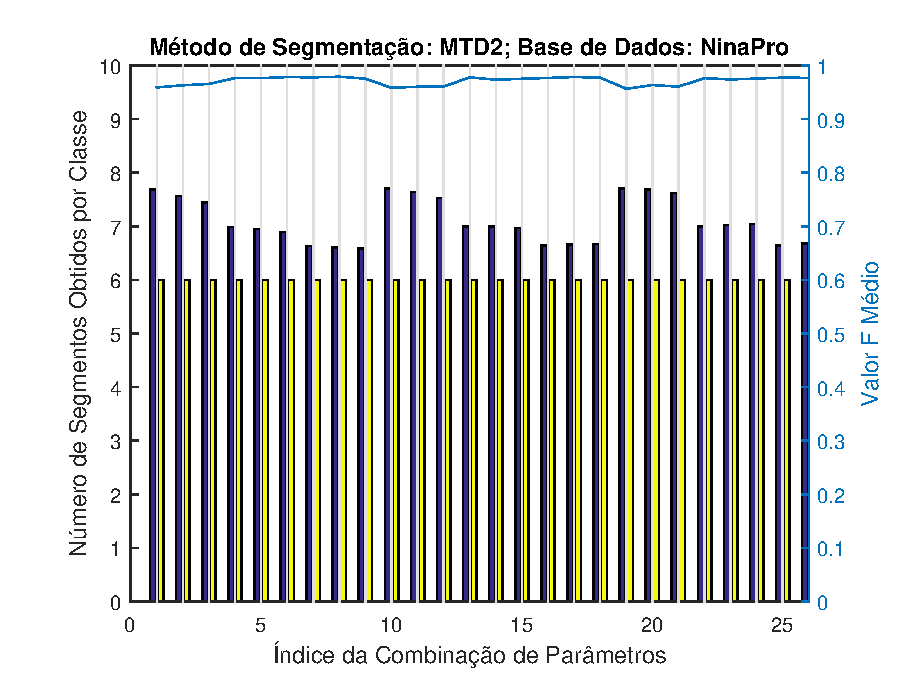
\includegraphics[width=0.75\linewidth]{./img/matlab/results/mtd2_nina.eps}
	\end{center}
	%\legend{Fonte: adaptado de BASMAJIAN \& DE LUCA, 1985}
\end{figure}

\begin{figure}[htb]
	\caption{\label{fig:mtd2Iee}Média e moda do número de segmentos obtidos por classe de movimento e valor $F$ médio de RNAs. Método de segmentação: MTD2. Base de dados: IEE}.
	\begin{center}
	    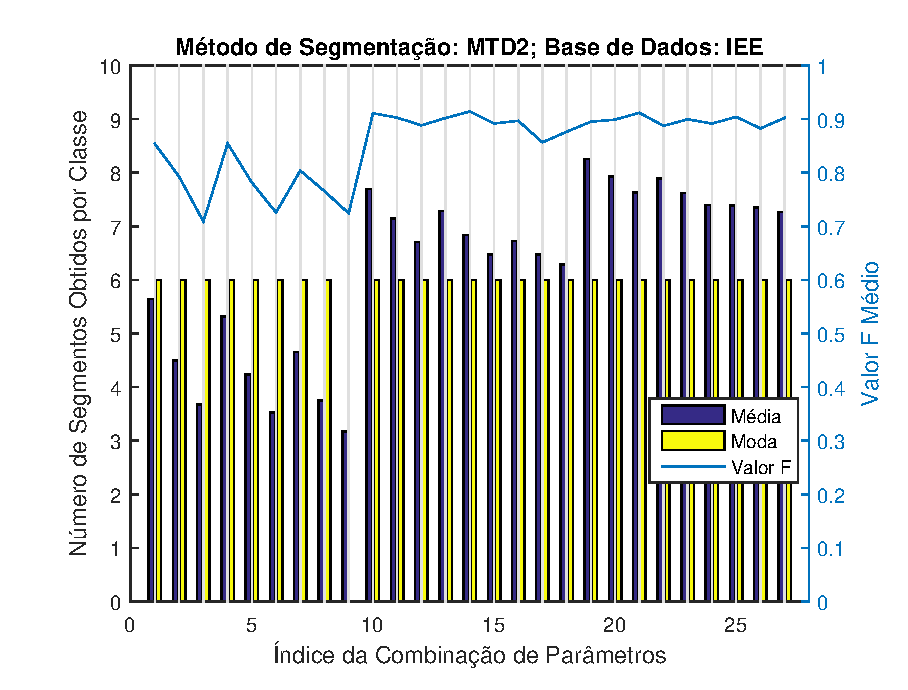
\includegraphics[width=0.75\linewidth]{./img/matlab/results/mtd2_iee.eps}
	\end{center}
	%\legend{Fonte: adaptado de BASMAJIAN \& DE LUCA, 1985}
\end{figure}

\begin{figure}[htb]
	\caption{\label{fig:mtd3Nina}Média e moda do número de segmentos obtidos por classe de movimento e valor $F$ médio de RNAs. Método de segmentação: MTD3. Base de dados: NinaPro}.
	\begin{center}
	    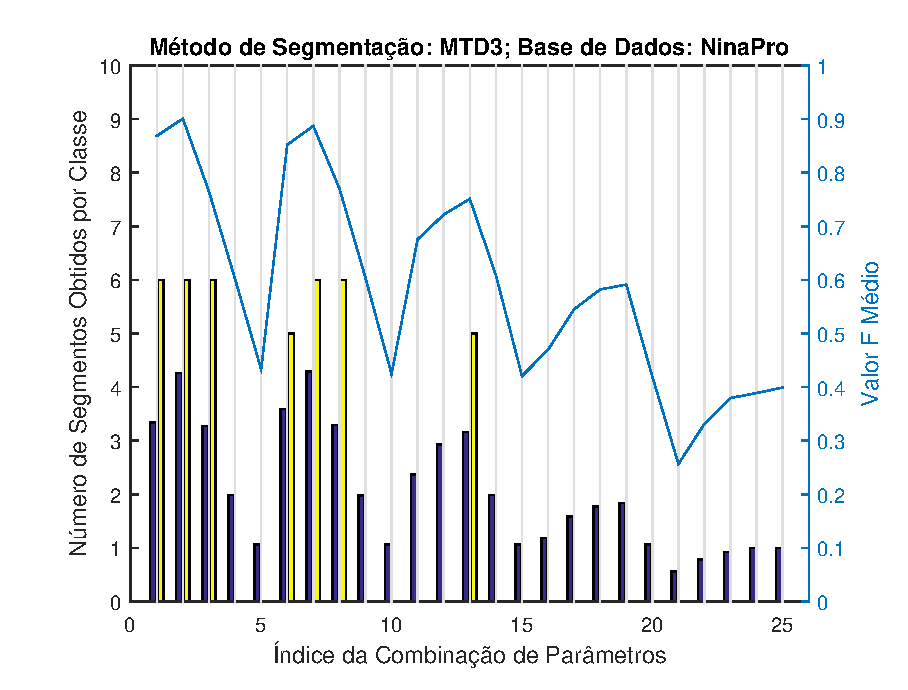
\includegraphics[width=0.75\linewidth]{./img/matlab/results/mtd3_nina.eps}
	\end{center}
	%\legend{Fonte: adaptado de BASMAJIAN \& DE LUCA, 1985}
\end{figure}

\begin{figure}[htb]
	\caption{\label{fig:mtd3Iee}Média e moda do número de segmentos obtidos por classe de movimento e valor $F$ médio de RNAs. Método de segmentação: MTD1. Base de dados: IEE}.
	\begin{center}
	    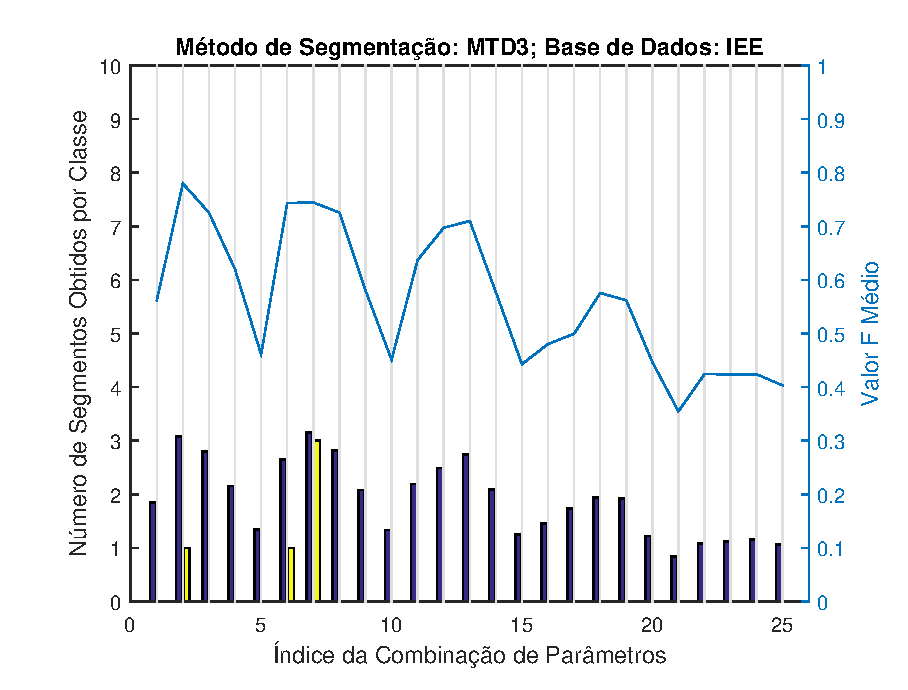
\includegraphics[width=0.75\linewidth]{./img/matlab/results/mtd3_iee.eps}
	\end{center}
	%\legend{Fonte: adaptado de BASMAJIAN \& DE LUCA, 1985}
\end{figure}

\begin{figure}[htb]
	\caption{\label{fig:mtd4Nina}Média e moda do número de segmentos obtidos por classe de movimento e valor $F$ médio de RNAs. Método de segmentação: MTD4. Base de dados: NinaPro}.
	\begin{center}
	    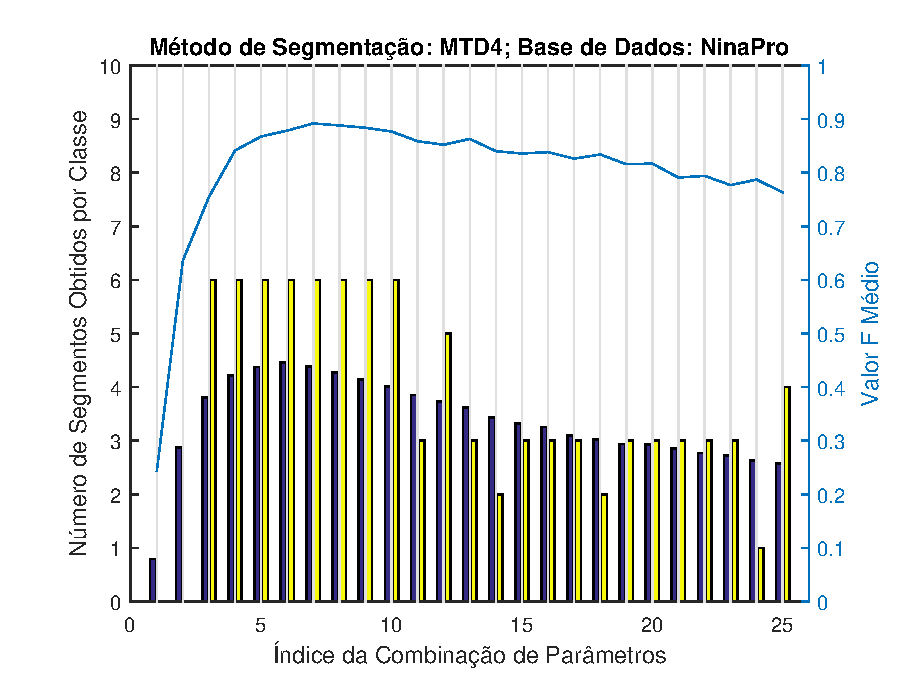
\includegraphics[width=0.75\linewidth]{./img/matlab/results/mtd4_nina.eps}
	\end{center}
	%\legend{Fonte: adaptado de BASMAJIAN \& DE LUCA, 1985}
\end{figure}

\begin{figure}[htb]
	\caption{\label{fig:mtd4Iee}Média e moda do número de segmentos obtidos por classe de movimento e valor $F$ médio de RNAs. Método de segmentação: MTD1. Base de dados: IEE}.
	\begin{center}
	    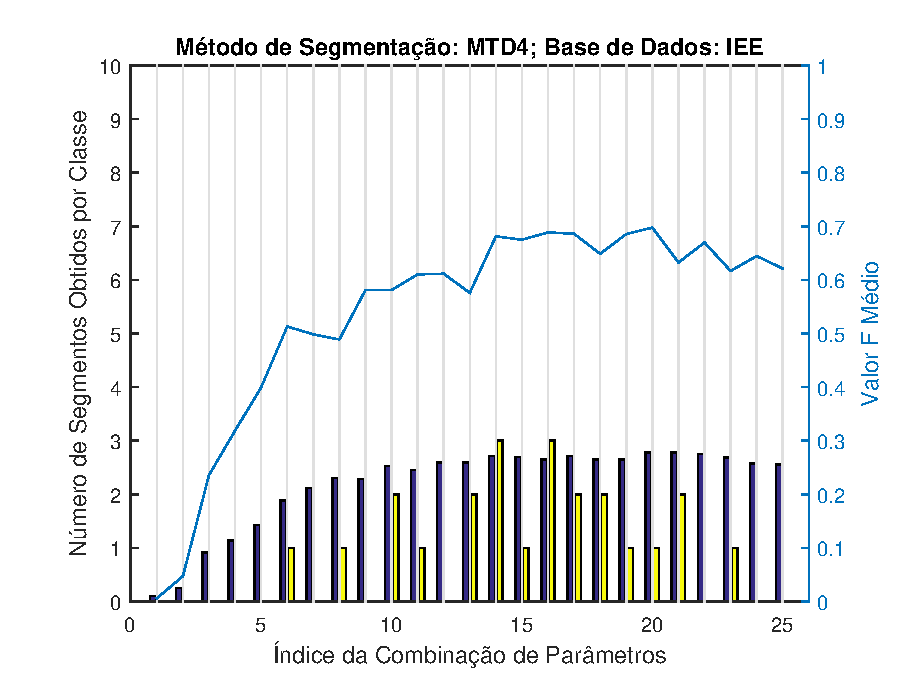
\includegraphics[width=0.75\linewidth]{./img/matlab/results/mtd4_iee.eps}
	\end{center}
	%\legend{Fonte: adaptado de BASMAJIAN \& DE LUCA, 1985}
\end{figure}

\textcolor{red}{TODO: finalizar análise}

%%-------------------------------------------------------------------------
%		\section{Classificação de Movimentos Utilizando RNAs}
%%-------------------------------------------------------------------------
%Para os resultados de segmentação obtidos com diferentes parâmetros testados apresentados nas Tabelas \ref{tab:num_mtd1_ninapro} a \ref{tab:number_mtd4_iee}, identificou-se as combinações de parâmetros que apresentaram os resultados de segmentação mais satisfatórios (i.e. parâmetros que segmentaram em seis partes cada movimento para o maior número possível de voluntários da base) para serem usados nos nos códigos dos apêndices \ref{ap:rna_mtd1} a \ref{ap:rna_mtd4}, que realizam segmentação e classificação de movimentos utilizando RNA. As combinações de parâmetros selecionadas são apresentadas na Tabela \ref{tab:chosen_params}.
%
%\begin{table}[htb]
\IBGEtab{\caption{\label{tab:chosen_params}Combinações de parâmetros selecionados para cada base de dados.}}
{
	\begin{tabular}{c|ccccc}
		\toprule
		Método 					& Base de dados	& Índice	& Parâmetros	&\pbox{2cm}{Média de \\ Segmentos por Classe}&\pbox{2cm}{Moda de \\ Segmentos por Classe}\\
		\midrule \midrule
		\multirow{2}{*}{MTD1}	& NinaPro		& 15 & $q = 0.95 \quad T_{lim} = 0.15$	&6,05&6\\
								& IEE			& 11 & $q = 0.75 \quad T_{lim} = 0.15$	&6,23&6\\
		\midrule                                                                             
		\multirow{2}{*}{MTD2}	& NinaPro		& 7	& $A = 60 \quad B = 8 \quad C = 2$	&6,01&6\\
								& IEE			& 18& $A = 100 \quad B = 8 \quad C = 5$	&6,28&6\\
		\midrule                                                                             
		\multirow{2}{*}{MTD3}	& NinaPro		& 7	& $B = 0.10 \quad C = -0.10$		&4,29&6\\
								& IEE			& 7 & $B = 0.10 \quad C = -0.10$		&3,15&3\\
		\midrule                                                                             
		\multirow{2}{*}{MTD4}	& NinaPro		& 6	& $T = 0.06$						&4,46&6\\
								& IEE			& 21& $T = 0.21$						&2,78&2\\
		\bottomrule
	\end{tabular}
}{}
\end{table}


%=========================================================================
% CONCLUSÃO
	\chapter{Conclusões}
%=========================================================================

%=========================================================================
% PROPOSTA DE TRABALHOS FUTUROS
	\chapter{Propostas de Trabalhos Futuros}
%=========================================================================

\textcolor{red}{PROPOSTAS: tradução dos códigos para outras linguagens (e.g. C++, Python); adaptação dos métodos para versões causais; aplicação no controle de prótese}

%=========================================================================
% REFERÊNCIAS BIBLIOGRÁFICAS
	\postextual
	\bibliography{referencias.bib}
%=========================================================================

%=========================================================================
% APÊNDICES
	\begin{apendicesenv}
	\partapendices
%=========================================================================
\chapter{Função em MATLAB para MTD1}
\lstinputlisting{../../MATLAB/seg_mtd1.m}
\label{ap:seg_mtd1}
%-------------------------------------------------------------------------
\chapter{Função em MATLAB para MTD2}
\lstinputlisting{../../MATLAB/seg_mtd2.m}
\label{ap:seg_mtd2}
%-------------------------------------------------------------------------
\chapter{Função em MATLAB para MTD3}
\lstinputlisting{../../MATLAB/seg_mtd3.m}
\label{ap:seg_mtd3}
%%-------------------------------------------------------------------------
\chapter{Função em MATLAB para MTD4}
\lstinputlisting{../../MATLAB/seg_mtd4.m}
\label{ap:seg_mtd4}
%-------------------------------------------------------------------------
\chapter{Código utilizado para determinação de $r_{target}$ do MTD1}
\label{ap:r_target}
\lstinputlisting{../../MATLAB/rtarget_mtd1.m}
%-------------------------------------------------------------------------
\chapter{Função em MATLAB para obtenção dos movimentos relacionados aos segmentos}
\label{ap:idMoves}
\lstinputlisting{../../MATLAB/identifyClasses.m}
%-------------------------------------------------------------------------
\end{apendicesenv}

%=========================================================================
% ANEXOS
	\begin{anexosenv}
	\partanexos
%=========================================================================
\chapter{Função em MATLAB para agrupamento com DBSCAN \cite{Thanh2013}}
\label{ap:dbscan}
\lstinputlisting{../../MATLAB/dbscan.m}
%-------------------------------------------------------------------------
\end{anexosenv}

\end{document}
